\documentclass[twocolumn]{aastex631}

\newcommand{\vdag}{(v)^\dagger}
\newcommand\aastex{AAS\TeX}
\newcommand\latex{La\TeX}
\usepackage{amsmath}
\usepackage{multirow}


\begin{document}

\title{Mapping Star Formation Quenching Efficiency Across Feedback and Cosmological Parameter Space with CAMELS Simulations}

\author{AstroPilot}
\affiliation{Anthropic, Gemini \& OpenAI servers. Planet Earth.}

\begin{abstract}
Understanding the mechanisms that halt star formation in galaxies, leading to their eventual quenching, is a fundamental problem in astrophysics. The challenge lies in disentangling the complex interplay between internal feedback processes, such as those driven by supernovae (SNe) and active galactic nuclei (AGN), and the influence of the larger cosmological environment. These processes are highly degenerate, making it difficult to isolate the specific drivers responsible for quenching. In this study, we address this challenge by systematically quantifying the impact of feedback and cosmological parameters on star formation quenching at $z=0$. We leverage the CAMELS simulation suite, a unique collection of hydrodynamical simulations designed to vary key astrophysical and cosmological parameters independently. By analyzing the relationships between galaxy properties and these parameters, we disentangle the relative importance of SNe, AGN feedback, and cosmological factors in regulating star formation and determine how they correlate with the quenched fraction of galaxies. Our analysis provides predictive insights for galaxy evolution models and offers a theoretical framework for interpreting future observational surveys aimed at understanding the quenching phenomenon, ultimately providing valuable constraints on the underlying physical processes driving galaxy evolution.
\end{abstract}

\keywords{Galaxy evolution, Galaxy quenching, Cosmological parameters, N-body simulations, Regression}


\section{Introduction}
\label{sec:intro}
Understanding the physical processes that govern the evolution of galaxies remains a central goal of modern astrophysics. Galaxies, as the primary repositories of stars, gas, and dark matter, exhibit a remarkable diversity in their properties, ranging from actively star-forming spirals to quiescent ellipticals with little to no ongoing star formation. A critical phase in the life cycle of a galaxy is the transition from an active star-forming state to a quenched state, where star formation is significantly suppressed or halted altogether. Elucidating the mechanisms that drive this quenching phenomenon is essential for a complete understanding of galaxy evolution and the formation of the diverse galaxy population we observe throughout cosmic history. This endeavor requires a synergistic approach, combining sophisticated theoretical models with detailed observational constraints.

The regulation of star formation in galaxies is a complex process influenced by a multitude of factors operating on different scales. Internal feedback processes, driven by supernovae (SNe) and active galactic nuclei (AGN), play a crucial role in shaping the gas content and star formation activity of galaxies \citep{hopkins2011selfregulatedstarformationgalaxies,carr2022regulationstarformationhot}. Supernovae inject energy and momentum into the interstellar medium (ISM), potentially heating and expelling gas, thereby suppressing star formation \citep{hopkins2011selfregulatedstarformationgalaxies,carr2022regulationstarformationhot}. Similarly, AGN can release vast amounts of energy in the form of radiation and outflows, which can also heat or remove gas from the galaxy, leading to quenching. These internal feedback mechanisms are intricately linked to the properties of the galaxy itself, such as its stellar mass, morphology, and gas content.

Furthermore, the larger cosmological environment in which a galaxy resides also exerts a significant influence on its star formation history \citep{wijesinghe2012galaxymassassemblygama,shi2023naturevsnurturerevisiting,pérezmillán2023relationmorphologystarformation}. Factors such as halo mass, merger history, and the density of the surrounding cosmic web can affect the inflow of fresh gas into galaxies, which fuels star formation \citep{wijesinghe2012galaxymassassemblygama,pérezmillán2023relationmorphologystarformation}. Environmental effects can also trigger morphological transformations, such as the formation of a bulge, which can stabilize gas against collapse and prevent star formation \citep{pérezmillán2023relationmorphologystarformation}. Disentangling the relative importance of these internal and external factors, and understanding how they interact to determine a galaxy's star formation history, presents a formidable challenge \citep{pérezmillán2023relationmorphologystarformation,mucesh2024natureversusnurturegalaxy}.

The observed properties of galaxies, such as their stellar mass, morphology, and star formation rate, represent the integrated outcome of these complex interactions  \citep{das2021galaxyinteractionsdifferentenvironments,li2024effectgalaxyinteractionsstarbursts}. This makes it difficult to isolate the specific drivers responsible for quenching based solely on observational data. Moreover, the theoretical modeling of these processes is computationally intensive, demanding high-resolution simulations that accurately capture the relevant physics on a wide range of scales  \citep{das2023galaxyinteractionsfilamentssheets,subramanian2023effectlowmassgalaxyinteractions}. Such simulations must faithfully reproduce both the internal physics of galaxies and their interaction with the larger cosmological environment.

To address these challenges, we present a systematic study aimed at quantifying the impact of feedback and cosmological parameters on star formation quenching at $z=0$  \citep{piotrowska2021quenchingstarformationobserved}. Our approach leverages the CAMELS (Cosmology and Astrophysics with MachinE Learning Simulations) simulation suite, a unique collection of hydrodynamical simulations specifically designed to independently vary key astrophysical and cosmological parameters. The CAMELS suite encompasses both the IllustrisTNG and SIMBA models, enabling us to explore the effects of different subgrid physics implementations on quenching. By analyzing the relationships between galaxy properties and these parameters, we aim to disentangle the relative importance of SNe, AGN feedback, and cosmological factors in regulating star formation  \citep{bluck2023fundamentalsignaturestarformation,kurinchivendhan2024originstarformationquenching}.

Our methodology involves a comprehensive analysis of the CAMELS simulation data, focusing on the quenched fraction of galaxies as a key indicator of quenching efficiency  \citep{xie2024quenchedgalaxieshow}. We employ a binning strategy to stratify galaxies by stellar mass and then further subdivide them based on the values of the feedback and cosmological parameters  \citep{xie2024quenchedgalaxieshow}. This allows us to isolate the effects of each parameter on the quenched fraction, while controlling for other factors  \citep{xie2024quenchedgalaxieshow}. Furthermore, we utilize statistical modeling techniques, such as multivariate logistic regression, to quantify the dependence of quenching efficiency on these parameters and to identify potential correlations and interactions. We model the quenched status of a galaxy as a binary variable, dependent on the input parameters  \citep{xie2024quenchedgalaxieshow}.

We derive several key metrics from our analysis, including the quenched fraction as a function of stellar mass and feedback/cosmological parameters \citep{xie2024quenchedgalaxieshow,xie2024quenchedgalaxieshow,geha2024sagasurveyivstar}, as well as the median specific star formation rate (sSFR) in each bin. We estimate the uncertainties on these metrics using bootstrap resampling techniques, providing a robust assessment of the statistical significance of our results. Additionally, we perform partial correlation analysis to isolate the direct effects of each parameter on the quenched fraction, controlling for stellar mass and other parameters \citep{porrasvalverde2024signatureblackholesquenched}. This allows us to identify the most influential factors driving quenching.

To validate our findings, we employ k-fold cross-validation techniques to assess the robustness of our regression models  \citep{narkedimilli2024predictingstellarmetallicitycomparative}. This ensures that our results are not driven by overfitting or sample variance. We also perform a series of robustness checks, repeating key analyses with alternative binning schemes and sSFR thresholds to confirm the stability of our conclusions  \citep{martin2024robustbayesianregressionastronomy,martin2024robustbayesianregressionastronomy}. These validation steps provide confidence in the reliability of our results and the generalizability of our findings  \citep{narkedimilli2024predictingstellarmetallicitycomparative,martin2024robustbayesianregressionastronomy,martin2024robustbayesianregressionastronomy}. We explore the parameter space and compare our findings to those of previous works to ensure our results are consistent with the current understanding of galaxy evolution  \citep{stoppa2023consistencytestscomparingastrophysical}.

Our analysis provides predictive insights for galaxy evolution models and offers a theoretical framework for interpreting future observational surveys aimed at understanding the quenching phenomenon  \citep{schawinski2018exploringgalaxyevolutiongenerative}. By quantifying the relative importance of different feedback and cosmological parameters, we can provide valuable constraints on the underlying physical processes driving galaxy evolution  \citep{lapi2025semiempiricalmodelsgalaxyformation}. This will help improve the accuracy and predictive power of galaxy evolution models, allowing them to better reproduce the observed properties of galaxies across cosmic time  \citep{li2024usinggalaxyevolutionsource}. The results can be used to improve the theoretical models which inform the observational surveys, and the observational surveys that improve the theoretical models  \citep{comparat2025crosscorrelationsoftxraysgalaxies}.

In future work, we plan to extend our analysis to higher redshifts, exploring the evolution of quenching efficiency over cosmic time \citep{mao2022revealingimpactsstellarmass,bravo2023galaxyquenchingtimescalesforensic}. This will provide a more complete picture of the quenching process and its dependence on feedback and cosmological parameters \citep{dou2025criticalroledarkmatter}. We also plan to investigate the role of different quenching mechanisms, such as morphological quenching and environmental quenching, in more detail \citep{mao2022revealingimpactsstellarmass,ellison2024galaxyevolutionpostmergerregime}. This will involve analyzing the morphology and environment of galaxies in the CAMELS simulations and correlating these properties with their star formation activity \citep{mao2022revealingimpactsstellarmass,bravo2023galaxyquenchingtimescalesforensic,ellison2024galaxyevolutionpostmergerregime}. Ultimately, this will lead to a more comprehensive understanding of the complex interplay between internal and external factors in regulating galaxy evolution.

\section{Methods}
\label{sec:methods}
\subsection{Data Acquisition and Preparation}
The foundation of this study rests upon the CAMELS (Cosmological and Astrophysical Models for Extremely Luminous Sources) project, a suite of cosmological hydrodynamical simulations. We utilize the publicly available data, specifically the IllustrisTNG and SIMBA simulation sets, each comprising 1000 simulations with varying cosmological and astrophysical parameters. The CAMELS simulations are particularly well-suited for this analysis due to their systematic variation of key parameters, enabling a disentangling of the effects of feedback and cosmology on galaxy evolution.

We begin by acquiring the galaxy-level data from the CAMELS database. This data is stored in \texttt{parquet} format for efficient storage and retrieval. Specifically, we load two primary dataframes: \texttt{galaxies\_full\_optimal.parquet}, containing detailed information on individual galaxies within the simulations, and \texttt{catalog\_params\_optimal.parquet}, providing the corresponding cosmological and feedback parameter values for each simulation. These dataframes are read into memory using the \texttt{pandas} library in Python, leveraging the \texttt{read\_parquet} function for optimized I/O performance.

The \texttt{galaxies\_full\_optimal.parquet} dataframe contains crucial information for each galaxy, including its star formation rate (SFR) and stellar mass (\texttt{M\_star}). The \texttt{catalog\_params\_optimal.parquet} dataframe contains the six parameters that are varied across the CAMELS simulations: two parameters controlling the efficiency of supernova feedback (\texttt{A\_SN1}, \texttt{A\_SN2}), two parameters controlling the efficiency of AGN feedback (\texttt{A\_AGN1}, \texttt{A\_AGN2}), the matter density parameter (\texttt{Omega\_m}), and the amplitude of the matter power spectrum (\texttt{sigma\_8}) \citep{villaescusanavarro2022camelsprojectpublicdata,lee2024zoomingcarpoolgplanenew}. Each simulation is uniquely identified by a \texttt{catalog\_number}.

\subsection{Calculation of Derived Quantities and Data Integration}
Following data loading, we compute the specific star formation rate (sSFR) for each galaxy, defined as the ratio of the SFR to the stellar mass (\texttt{sSFR = SFR / M\_star}) \citep{bauer2005specificstarformationrates}. This quantity serves as a key indicator of a galaxy's star-forming activity. We then define a galaxy as "quenched" if its sSFR falls below a threshold of $10^{-11}$ yr$^{-1}$ \citep{whitaker2017predictingquiescencedependencespecific,katsianis2020specificstarformationrate,leslie2020vlacosmos3ghzlarge}. A boolean column is added to the galaxy dataframe, indicating whether each galaxy meets this quenching criterion.

To link galaxy-level properties with the corresponding simulation parameters, we merge the \texttt{catalog\_params\_optimal.parquet} dataframe onto the \texttt{galaxies\_full\_optimal.parquet} dataframe using the \texttt{catalog\_number} as the common key. This ensures that each galaxy is associated with the correct values of \texttt{A\_SN1}, \texttt{A\_SN2}, \texttt{A\_AGN1}, \texttt{A\_AGN2}, \texttt{Omega\_m}, and \texttt{sigma\_8} from its parent simulation \citep{contardo2025effectsparametersgalaxyproperties}. The merging operation is performed using the \texttt{merge} function in \texttt{pandas} \citep{desanti2025fieldlevelsimulationbasedinferencegalaxy,ivanov2025fullshapeanalysissimulationbasedpriors}.

\subsection{Binning Strategy for Parameter Space Exploration}
To systematically explore the influence of stellar mass, feedback, and cosmological parameters on quenching, we employ a binning strategy. First, galaxies are divided into bins based on their stellar mass. We utilize logarithmic bins, specifically log(\texttt{M\_star}/M$_\odot$) = [8.5–9.5], [9.5–10.5], and [10.5–11.5] \citep{porrasvalverde2024signatureblackholesquenched}. These bins are chosen to ensure sufficient galaxy counts within each bin, providing robust statistical analysis.

Within each stellar mass bin, we further stratify galaxies based on the feedback and cosmological parameters \citep{vaughan2024samigalaxysurveypredicting}. For the feedback parameters (\texttt{A\_SN1}, \texttt{A\_SN2}, \texttt{A\_AGN1}, \texttt{A\_AGN2}) and the cosmological parameters (\texttt{Omega\_m}, \texttt{sigma\_8}), we divide their respective ranges into quantiles \citep{arangotoro2025cosmoswebhistorygalaxymigrations}. This approach ensures a uniform sampling across the parameter space, even if the underlying distributions are non-uniform. We experiment with different numbers of quantiles (e.g., quartiles or quintiles) to optimize the balance between resolution and statistical power.

For higher-order analysis, we explore the use of two-dimensional binning (e.g., \texttt{A\_SN1} vs. \texttt{A\_AGN1}) to capture potential interactions between parameters \citep{cappellari2002adaptivespatialbinning2d,cappellari2003adaptivespatialbinningintegralfield,cappellari2009voronoibinningoptimaladaptive}. In cases where multi-dimensional binning leads to sparse bins, we employ regression techniques to disentangle the effects of individual parameters without excessive binning.

\subsection{Calculation of Quenching Metrics and Uncertainty Estimation}
For each combination of stellar mass bin and parameter bin, we calculate the quenched fraction (\texttt{f\_quenched}), defined as the number of quenched galaxies (\texttt{N\_quenched}) divided by the total number of galaxies (\texttt{N\_total}) within that bin \citep{xie2024quenchedgalaxieshow}.
\begin{equation}
f_{\text{quenched}} = \frac{N_{\text{quenched}}}{N_{\text{total}}}
\end{equation}
In addition to the quenched fraction, we also compute the median sSFR within each bin to provide a continuous measure of star-forming activity \citep{banerjee2023clusteringphysicalpropertiesstarforming,shi2023naturevsnurturerevisiting}.

To quantify the uncertainties associated with the quenched fraction and median sSFR, we employ a bootstrap resampling technique \citep{sanderson2009xraymodellinggalaxycluster,mohammad2022creatingjackknifebootstrapestimates}. Within each bin, we resample galaxies with replacement a large number of times (e.g., 1000 times). For each resampled dataset, we recalculate the quenched fraction and median sSFR. The standard deviation of these resampled values is then used as an estimate of the uncertainty for each metric \citep{sanderson2009xraymodellinggalaxycluster,mohammad2022creatingjackknifebootstrapestimates}.

\subsection{Statistical Modeling and Regression Analysis}
To quantify the dependence of quenching efficiency on feedback and cosmological parameters, we perform multivariate logistic regression \citep{kuschel2023investigatingdominantenvironmentalquenching,xie2024quenchedgalaxieshow,rutkowski2025recentstarformation05z15}. The dependent variable is the quenched status of a galaxy (a binary variable indicating whether a galaxy is quenched or not), and the independent variables are the feedback parameters (\texttt{A\_SN1}, \texttt{A\_SN2}, \texttt{A\_AGN1}, \texttt{A\_AGN2}), the cosmological parameters (\texttt{Omega\_m}, \texttt{sigma\_8}), and the logarithm of the stellar mass (log(\texttt{M\_star})). The logistic regression model takes the form:
\begin{equation}
\text{logit}(p) = \beta_0 + \beta_1 A_{\text{SN1}} + \beta_2 A_{\text{SN2}} + \beta_3 A_{\text{AGN1}} + \beta_4 A_{\text{AGN2}} + \beta_5 \Omega_m + \beta_6 \sigma_8 + \beta_7 \log(M_{\text{star}}) + \dots
\end{equation}
where \( p \) is the probability of a galaxy being quenched, \( \beta_i \) are the regression coefficients, and the ellipsis indicates the potential inclusion of interaction terms \citep{romerogómez2024earlytypegalaxiesquenchedpresentday,zheng2025photometricobjectscosmicwebs}.

We also consider the inclusion of interaction terms (e.g., \texttt{A\_SN1} $\times$ \texttt{A\_AGN1}) in the regression model to capture potential non-linear effects and dependencies between parameters \citep{llorella2025exploringsymbolicregressiongenetic,tian2025interactivesymbolicregressionoffline}.

To isolate the direct effects of each parameter on the quenched fraction, we compute partial correlations between each parameter and the quenched fraction, controlling for stellar mass and the other parameters \citep{porrasvalverde2024signatureblackholesquenched}.

\subsection{Model Validation and Robustness Checks}
To assess the robustness of the regression results, we employ k-fold cross-validation \citep{hammond2024identifyingfittingeclipsemaps,sweet2024predictingexoplanetaryfeaturesresidual}. We divide the data into k folds (e.g., k=5) \citep{sweet2024predictingexoplanetaryfeaturesresidual}. For each fold, we fit the model on the remaining k-1 folds (the training set) and test its performance on the held-out fold (the testing set) \citep{sweet2024predictingexoplanetaryfeaturesresidual}. We repeat this process for each of the k folds, and record performance metrics such as accuracy and area under the receiver operating characteristic curve (AUC) \citep{hammond2024identifyingfittingeclipsemaps,sweet2024predictingexoplanetaryfeaturesresidual}. The cross-validation provides an estimate of the model's generalization performance and helps to prevent overfitting \citep{hammond2024identifyingfittingeclipsemaps,sweet2024predictingexoplanetaryfeaturesresidual}.

We also perform robustness checks by repeating key analyses with alternative binning schemes \citep{leslie2021modebymoderelativebinningfast,dainotti2024newbinningmethodchoose,chen2024evolutionxraygalaxycluster} and sSFR thresholds to confirm the stability of the results.

\subsection{Computational Implementation}
All data processing, analysis, and visualization are performed using Python, leveraging libraries such as \texttt{pandas}, \texttt{numpy}, \texttt{scikit-learn}, \texttt{matplotlib}, and \texttt{seaborn} \citep{giri2025astronomycalcpythontoolkitteaching}. Vectorized operations in \texttt{pandas} and \texttt{numpy} are used extensively to optimize computational efficiency \citep{turk2011highperformanceastrophysicalsimulationsanalysis}. For computationally intensive tasks such as bootstrap resampling and cross-validation, we leverage parallel processing using Python's \texttt{concurrent.futures} module to utilize all available CPU cores \citep{turk2011highperformanceastrophysicalsimulationsanalysis}.

\section{Results}
\label{sec:results}
\subsection{Quenched Fraction Trends}

This section presents a detailed analysis of star formation quenching efficiency across the CAMELS simulation suite, focusing on the impact of supernova (SN) and active galactic nucleus (AGN) feedback parameters, as well as cosmological parameters. We explore trends in quenched fractions, examine the relative importance of each parameter using statistical modeling, and investigate the interplay between these factors in driving galaxy quenching at \(z=0\).

\subsubsection{Stellar Mass Dependence}

We begin by examining the quenched fraction (\(f_{quenched}\)), defined as the fraction of galaxies with specific star formation rate (sSFR) below \(10^{-11} \text{ yr}^{-1}\), as a function of stellar mass and the varied simulation parameters. The distribution of sSFR for quenched and star-forming galaxies is shown in Figure \ref{fig:sSFR_hist}, illustrating a clear separation between the two populations. The stellar mass distributions for quenched and star-forming galaxies are shown in Figure \ref{fig:Mstar_hist}, indicating that star-forming galaxies tend to have lower stellar masses than quenched galaxies. Galaxies are binned into stellar mass ranges of width one dex.

A strong positive correlation exists between stellar mass and quenched fraction. In the highest mass bin considered, \(10.5 \leq \log_{10}(M_{star}/M_\odot) < 11.5\), \(f_{quenched}\) consistently exceeds 0.8 across all feedback parameter values. This indicates that galaxies in this mass range are nearly universally quenched, irrespective of the specific feedback implementation. In contrast, the quenched fraction varies significantly with feedback parameters in lower mass bins.

\begin{figure}[h!]
    \centering
    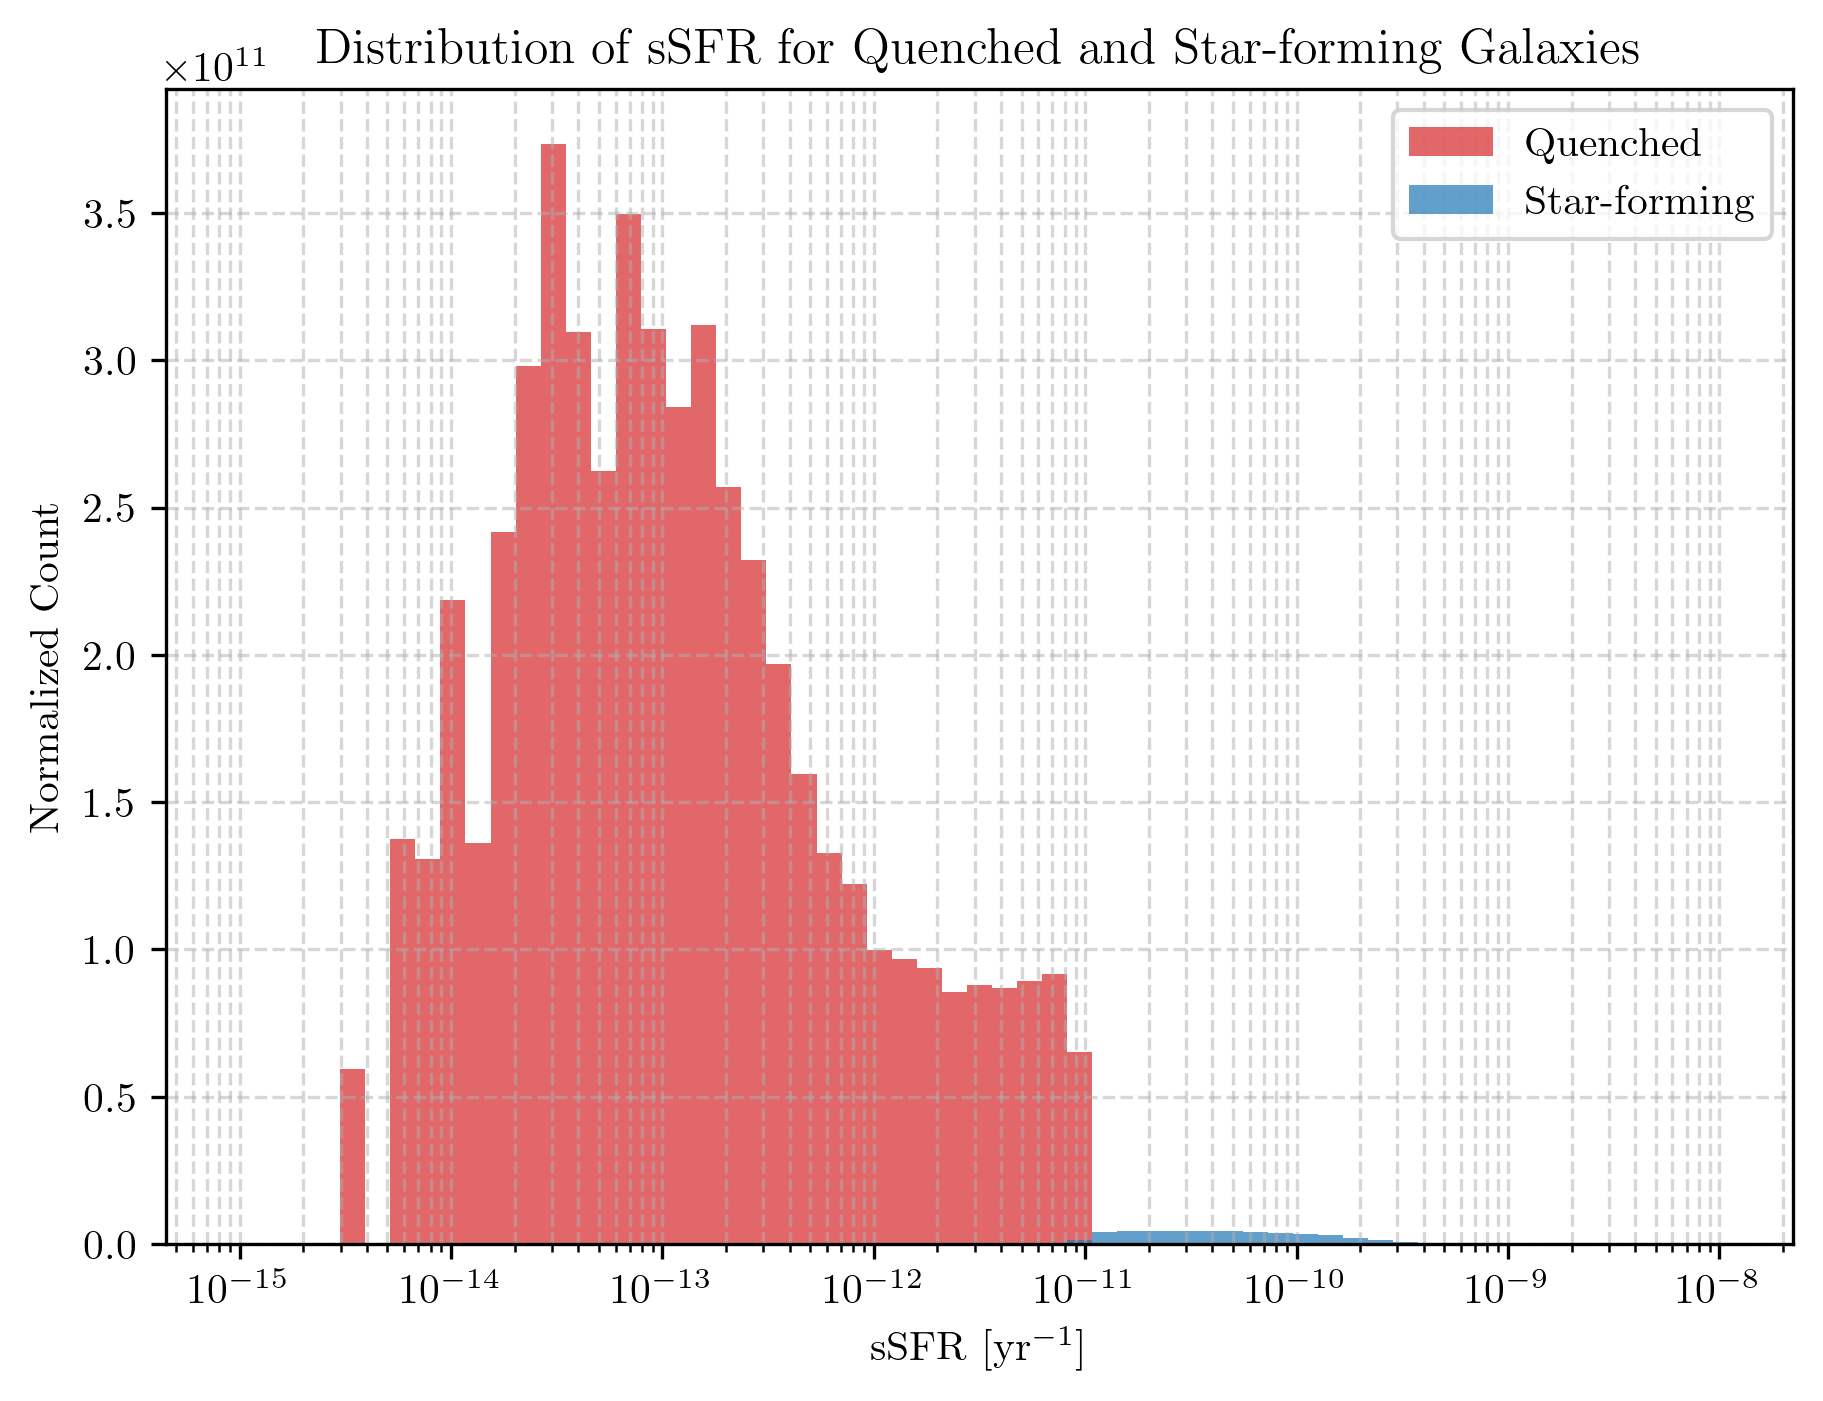
\includegraphics[width=0.5\textwidth]{../Project6/plots/sSFR_histogram_1_20250424_133143.png}
    \caption{\label{fig:sSFR_hist} Distribution of specific star formation rates (sSFR) for quenched and star-forming galaxies. A clear separation is observed between the two populations, with quenched galaxies exhibiting significantly lower sSFR values compared to star-forming galaxies. The quenched galaxies have a higher normalized count at lower sSFR values.
}
\end{figure}

\begin{figure}[h!]
    \centering
    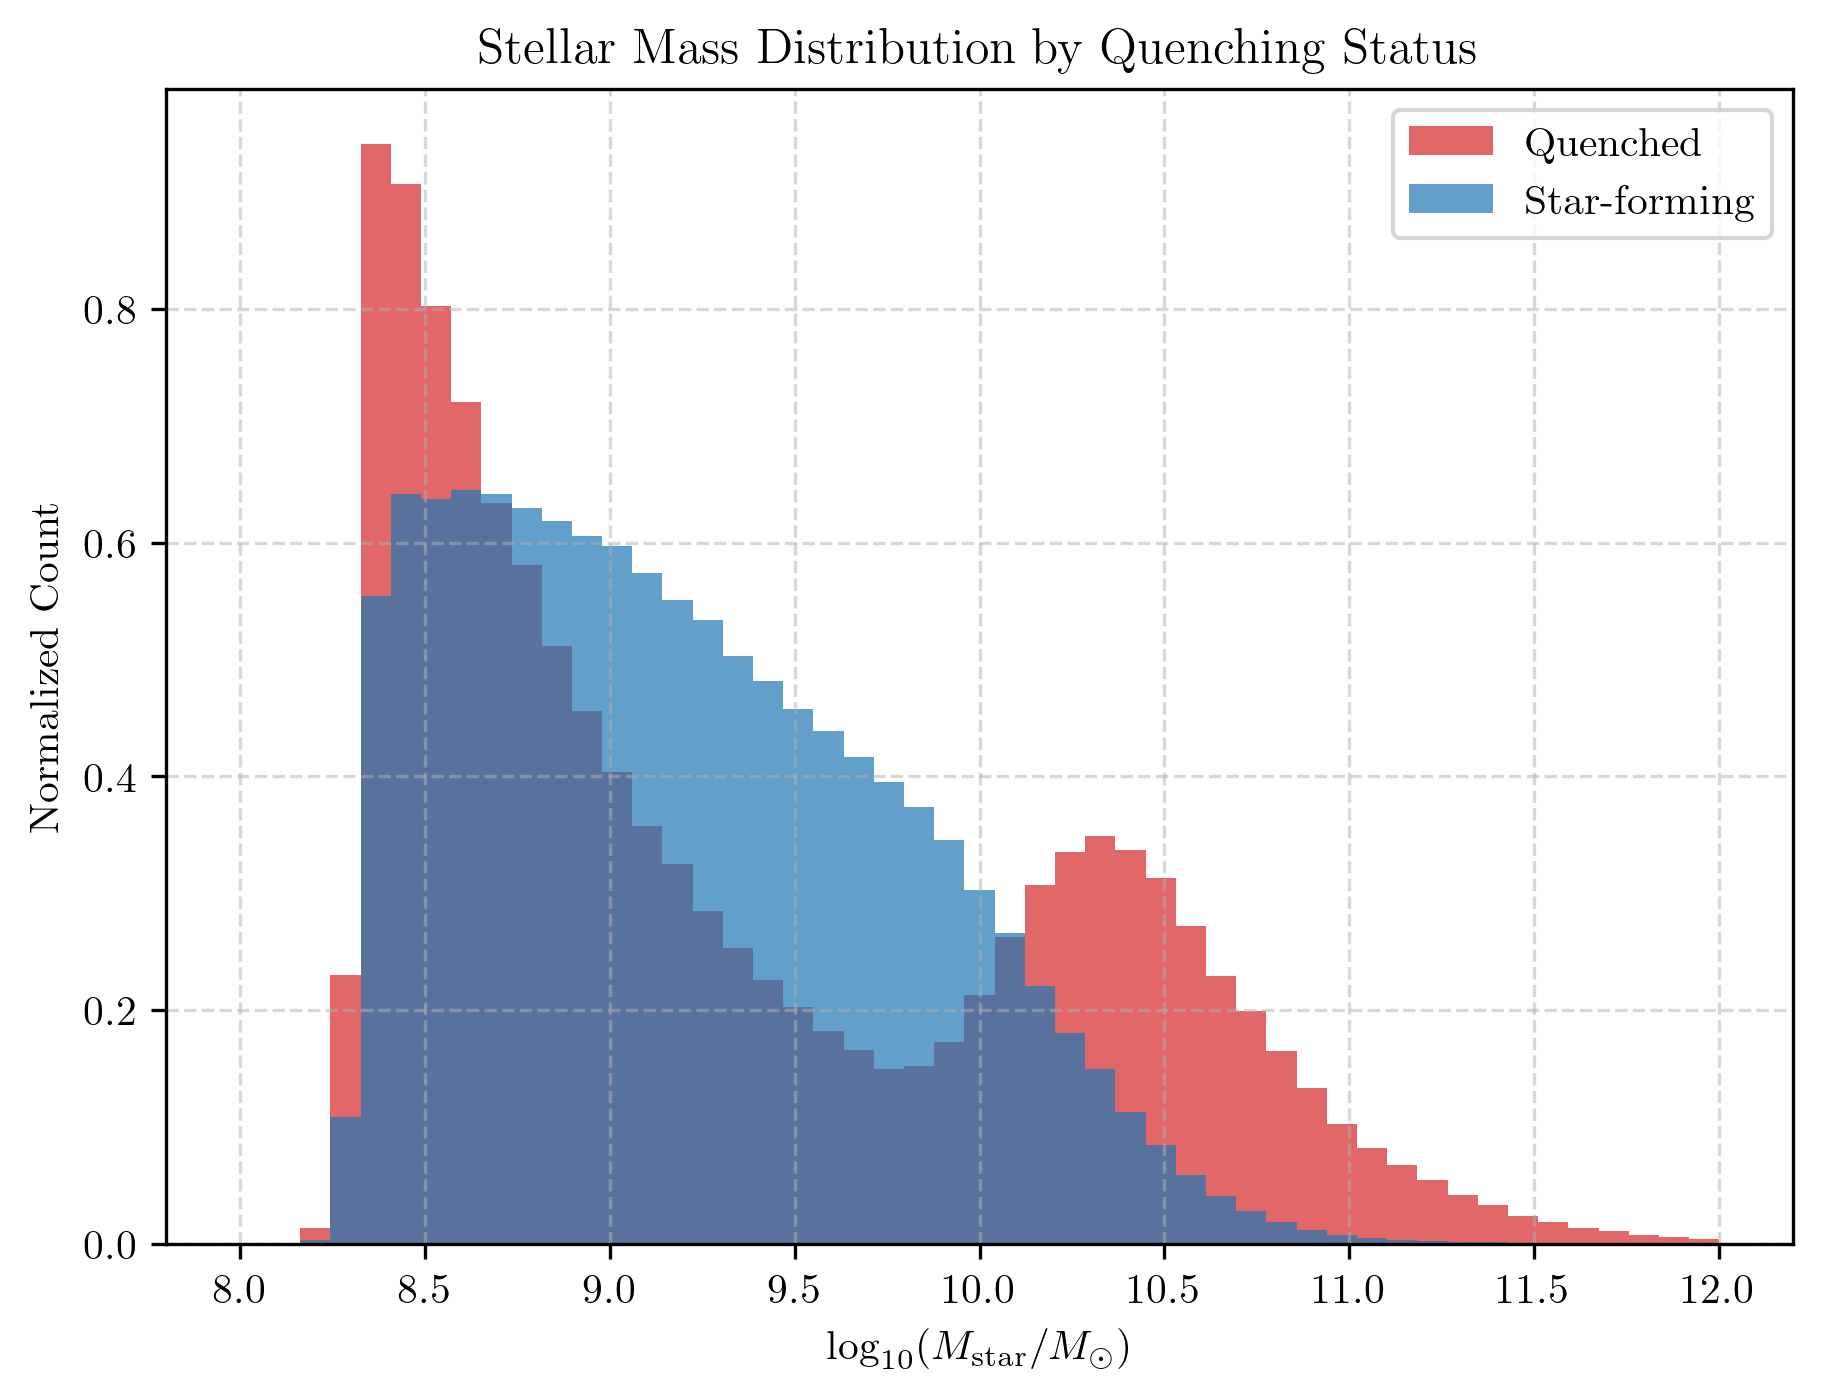
\includegraphics[width=0.5\textwidth]{../Project6/plots/Mstar_histogram_2_20250424_133143.png}
    \caption{\label{fig:Mstar_hist} The figure shows the stellar mass distribution, separated by quenching status. The red histogram represents quenched galaxies, while the blue histogram represents star-forming galaxies. The x-axis shows the logarithm of the stellar mass in solar masses, and the y-axis shows the normalized count. There are large differences in the distributions, with star-forming galaxies peaking at lower stellar masses than quenched galaxies.
}
\end{figure}

\subsubsection{Supernova Feedback}

The parameter \(A_{SN1}\), representing the SN wind energy per unit star formation rate, exhibits a notable *negative* correlation with \(f_{quenched}\) in low to intermediate mass galaxies. This trend is illustrated in Figure \ref{fig:fquenched_ASN1}, where the quenched fraction is plotted against \(A_{SN1}\) for different stellar mass bins. Specifically, for galaxies in the lowest mass bin (\(9.5 \leq \log_{10}(M_{star}/M_\odot) < 10.5\)), \(f_{quenched}\) decreases from approximately 0.40 in the lowest quartile of \(A_{SN1}\) values to around 0.24 in the highest quartile. This suggests that enhanced SN feedback can suppress quenching, potentially by maintaining a turbulent interstellar medium (ISM) and preventing the collapse of gas clouds necessary for sustained star formation. The distribution of $A_{SN1}$ for quenched and star-forming galaxies is shown in Figure \ref{fig:ASN1_hist}, further highlighting the differences between the two populations.

\begin{figure}[h!]
    \centering
    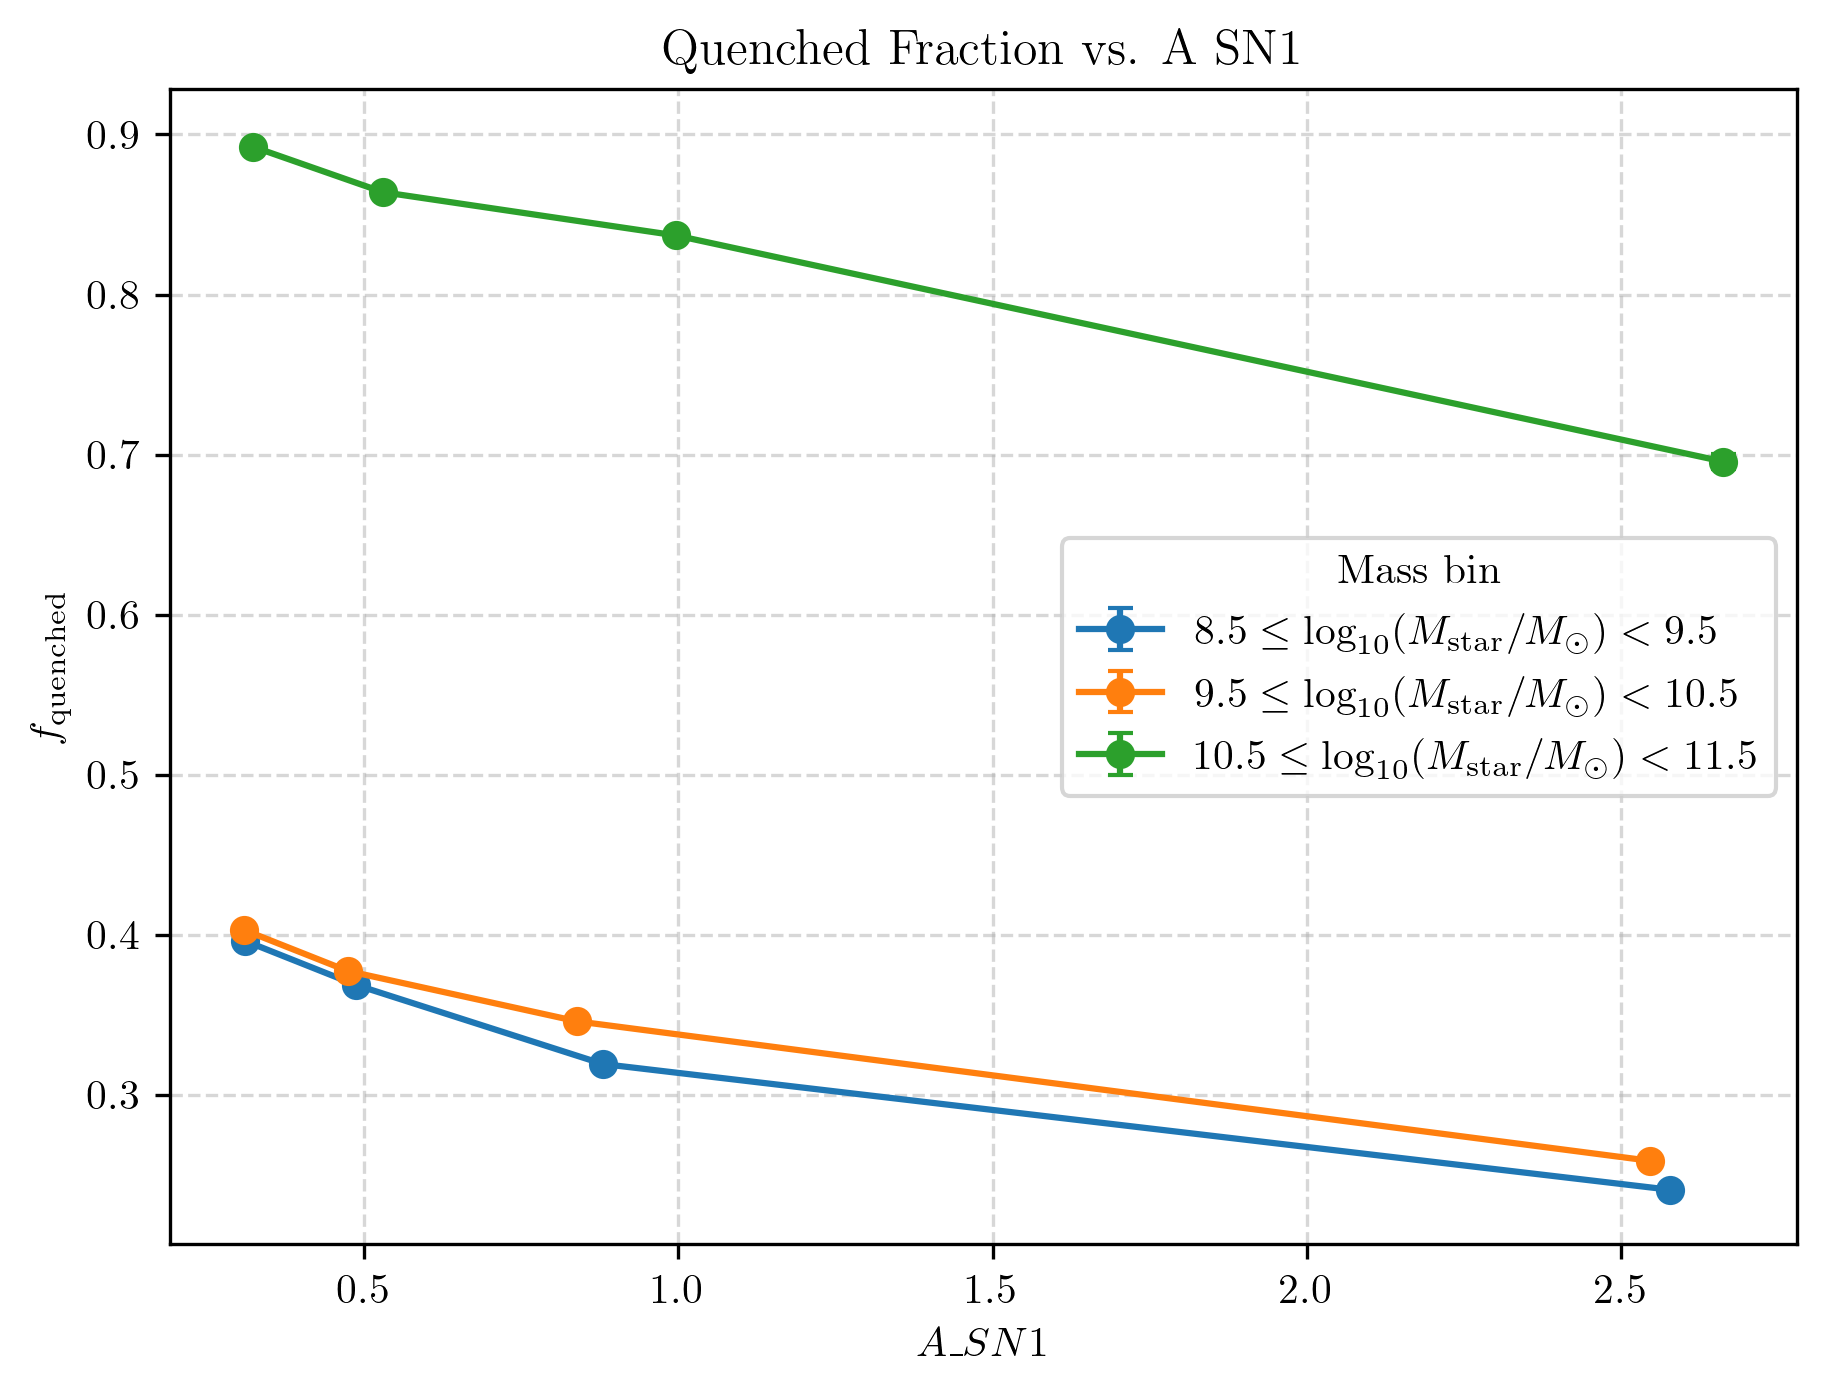
\includegraphics[width=0.5\textwidth]{../Project6/plots/fquenched_vs_A_SN1_20250424_133824.png}
    \caption{\label{fig:fquenched_ASN1} The figure shows the quenched fraction as a function of $A_{SN1}$ for three different stellar mass bins: $8.5 \leq \log_{10}(M_{star}/M_{\odot}) < 9.5$, $9.5 \leq \log_{10}(M_{star}/M_{\odot}) < 10.5$, and $10.5 \leq \log_{10}(M_{star}/M_{\odot}) < 11.5$. The quenched fraction decreases with increasing $A_{SN1}$ for all mass bins. At a given $A_{SN1}$, the quenched fraction is higher for more massive galaxies.
}
\end{figure}

\begin{figure}[h!]
    \centering
    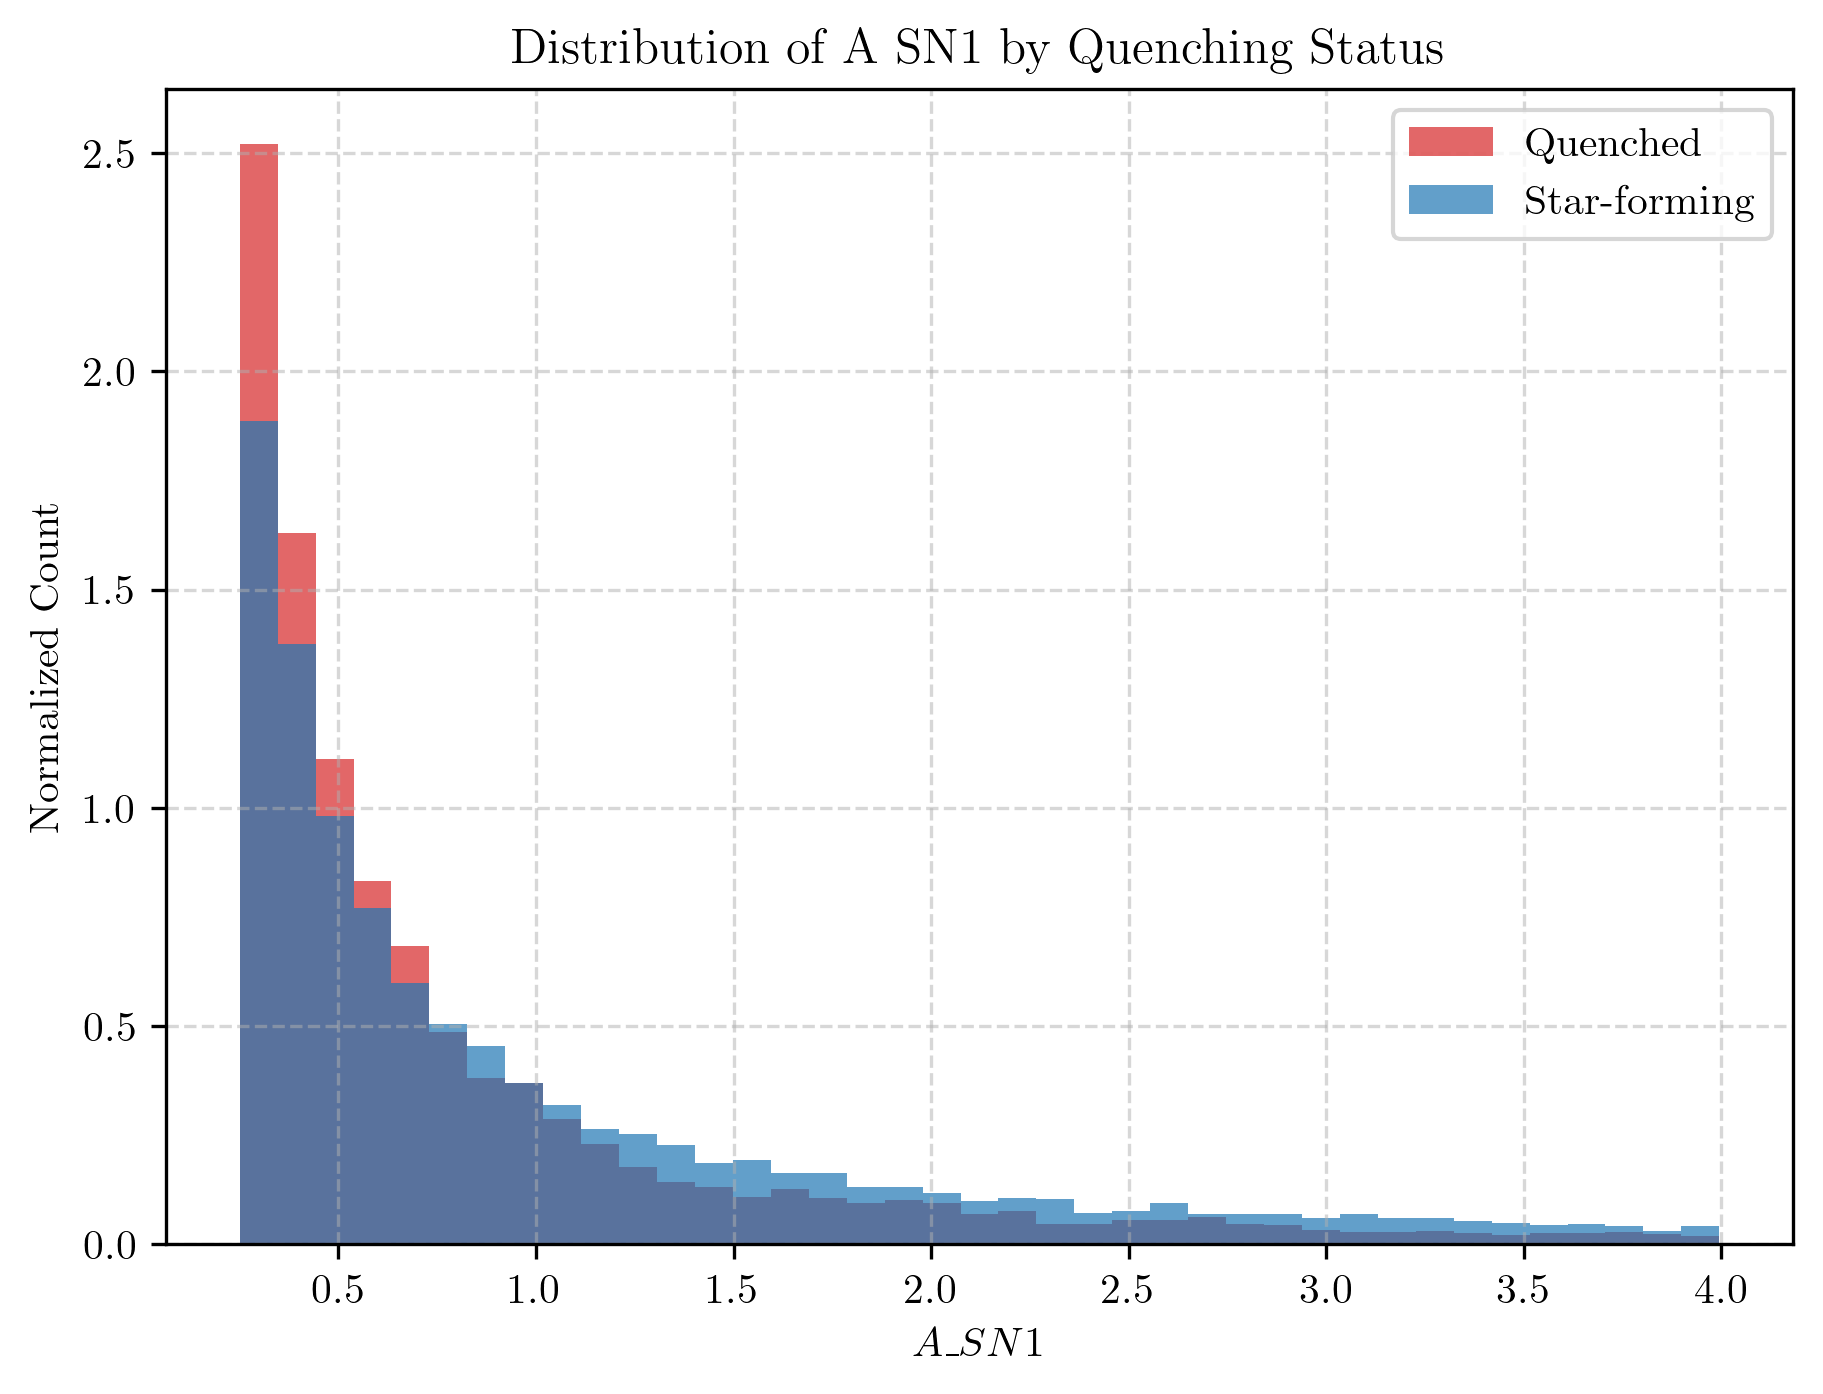
\includegraphics[width=0.5\textwidth]{../Project6/plots/A_SN1_histogram_3_20250424_133143.png}
    \caption{\label{fig:ASN1_hist} Distribution of $A_{SN1}$ for quenched and star-forming galaxies. The plot shows the normalized count of $A_{SN1}$ values, with quenched galaxies indicated in red and star-forming galaxies in blue. The distribution of $A_{SN1}$ exhibits differences between the two types of galaxies.
}
\end{figure}

\subsubsection{AGN Feedback}

Conversely, the AGN feedback parameter \(A_{AGN1}\), representing the AGN feedback energy per unit accretion rate, displays a positive correlation with \(f_{quenched}\) across all mass bins. This trend is visible in Figure \ref{fig:fquenched_AAGN1}, which shows the quenched fraction as a function of $A_{AGN1}$ for different stellar mass bins. For example, in the highest mass bin, \(f_{quenched}\) increases from approximately 0.72 in the lowest quartile of \(A_{AGN1}\) to approximately 0.94 in the highest quartile. Figure \ref{fig:AAGN1_hist} shows the distribution of $A_{AGN1}$ for quenched and star-forming galaxies, illustrating the higher $A_{AGN1}$ values for quenched galaxies. This result supports the established paradigm that AGN feedback plays a critical role in maintaining quenching in massive galaxies, by heating and/or expelling the gas reservoir.

\begin{figure}[h!]
    \centering
    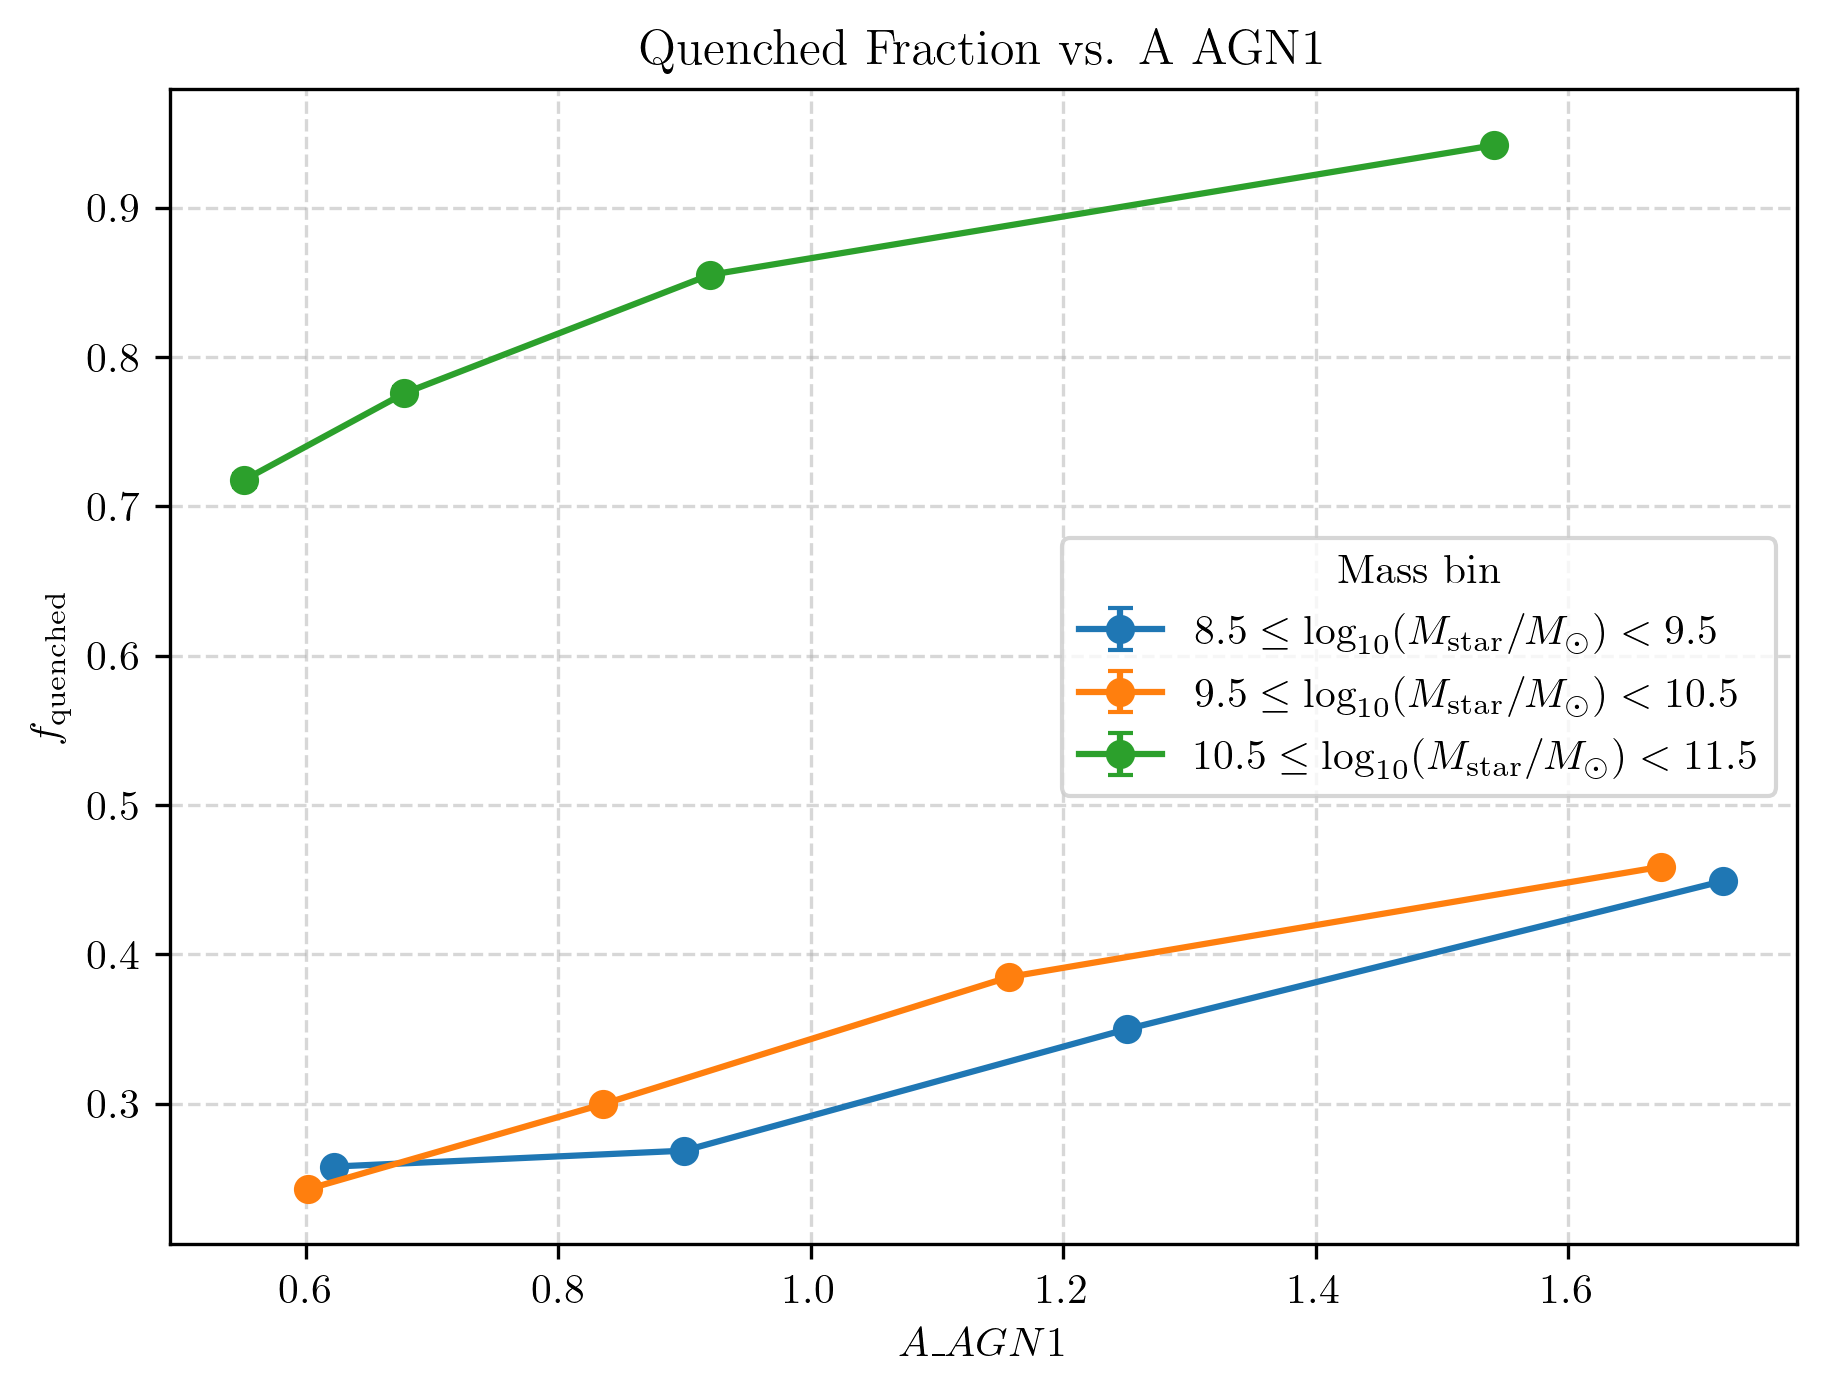
\includegraphics[width=0.5\textwidth]{../Project6/plots/fquenched_vs_A_AGN1_20250424_133935.png}
    \caption{\label{fig:fquenched_AAGN1} Quenched fraction as a function of A\ensuremath{\_}AGN1 for different stellar mass bins. The quenched fraction increases with increasing A\ensuremath{\_}AGN1, with large differences seen between the different stellar mass bins.
}
\end{figure}

\begin{figure}[h!]
    \centering
    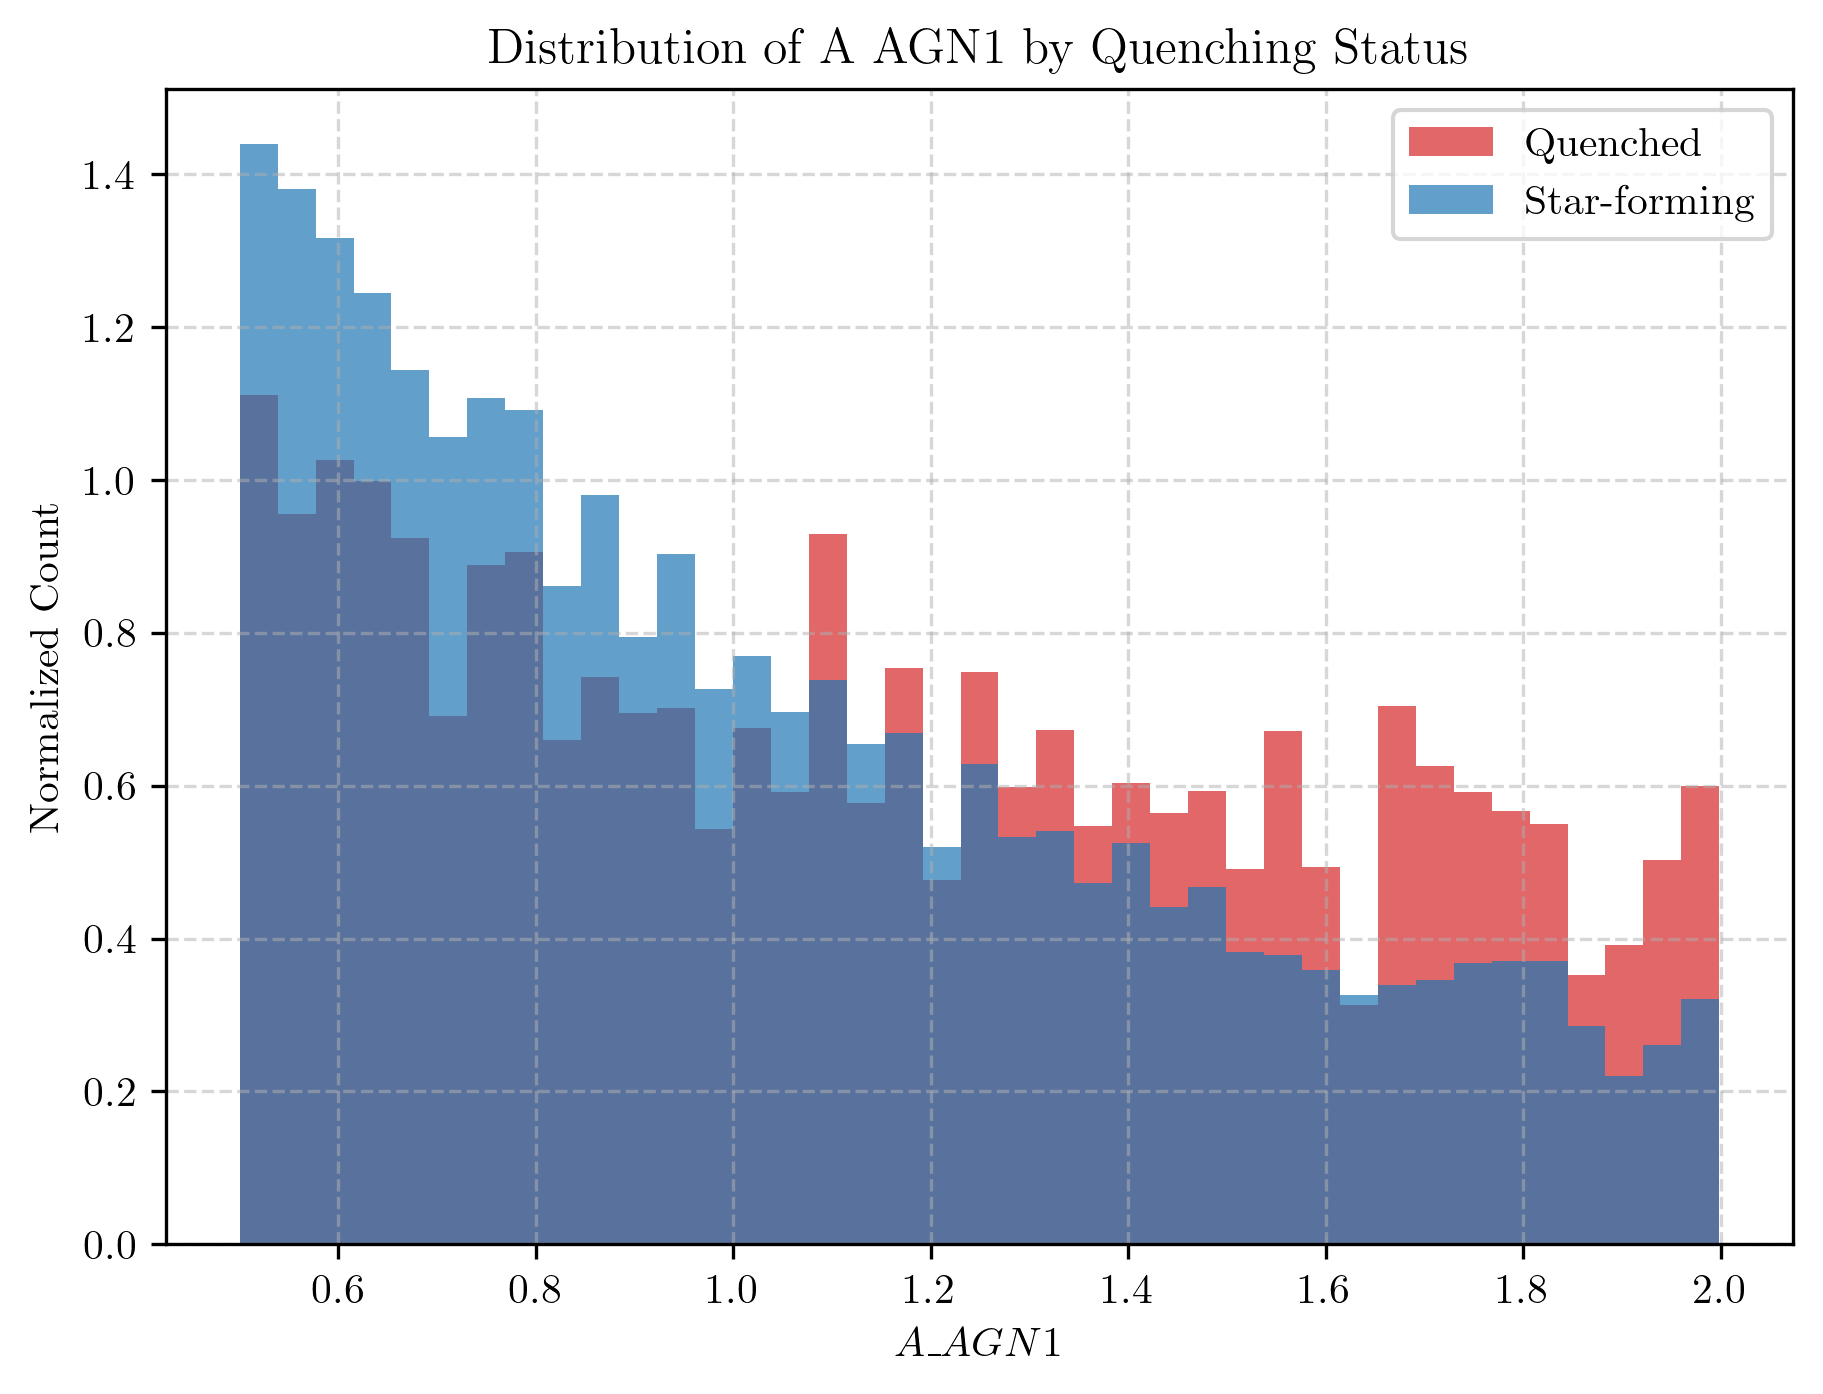
\includegraphics[width=0.5\textwidth]{../Project6/plots/A_AGN1_histogram_5_20250424_133143.png}
    \caption{\label{fig:AAGN1_hist} The distribution of $A\_AGN1$ is shown, separated by quenching status. Star-forming galaxies are shown in blue, while quenched galaxies are shown in red. There are large differences between the two populations with quenched galaxies having higher $A\ensuremath{\_}AGN1$ values.
}
\end{figure}

\subsubsection{Other Feedback Parameters}

The parameters \(A_{SN2}\) (SN wind speed) and \(A_{AGN2}\) (AGN kinetic mode ejection speed) show weaker and less systematic trends compared to \(A_{SN1}\) and \(A_{AGN1}\). Figure \ref{fig:fquenched_ASN2} shows the quenched fraction as a function of $A_{SN2}$ for different stellar mass bins, indicating a weak dependence. Similarly, Figure \ref{fig:fquenched_AAGN2} shows the quenched fraction as a function of $A_{AGN2}$, also showing a weak dependence. The distributions of $A_{SN2}$ and $A_{AGN2}$ for quenched and star-forming galaxies are shown in Figure \ref{fig:ASN2_hist} and Figure \ref{fig:AAGN2_hist}, respectively. This suggests that the overall energy injected by feedback processes is more crucial for regulating quenching than the specific velocity of the outflows, at least within the parameter ranges explored in this study.

\begin{figure}[h!]
    \centering
    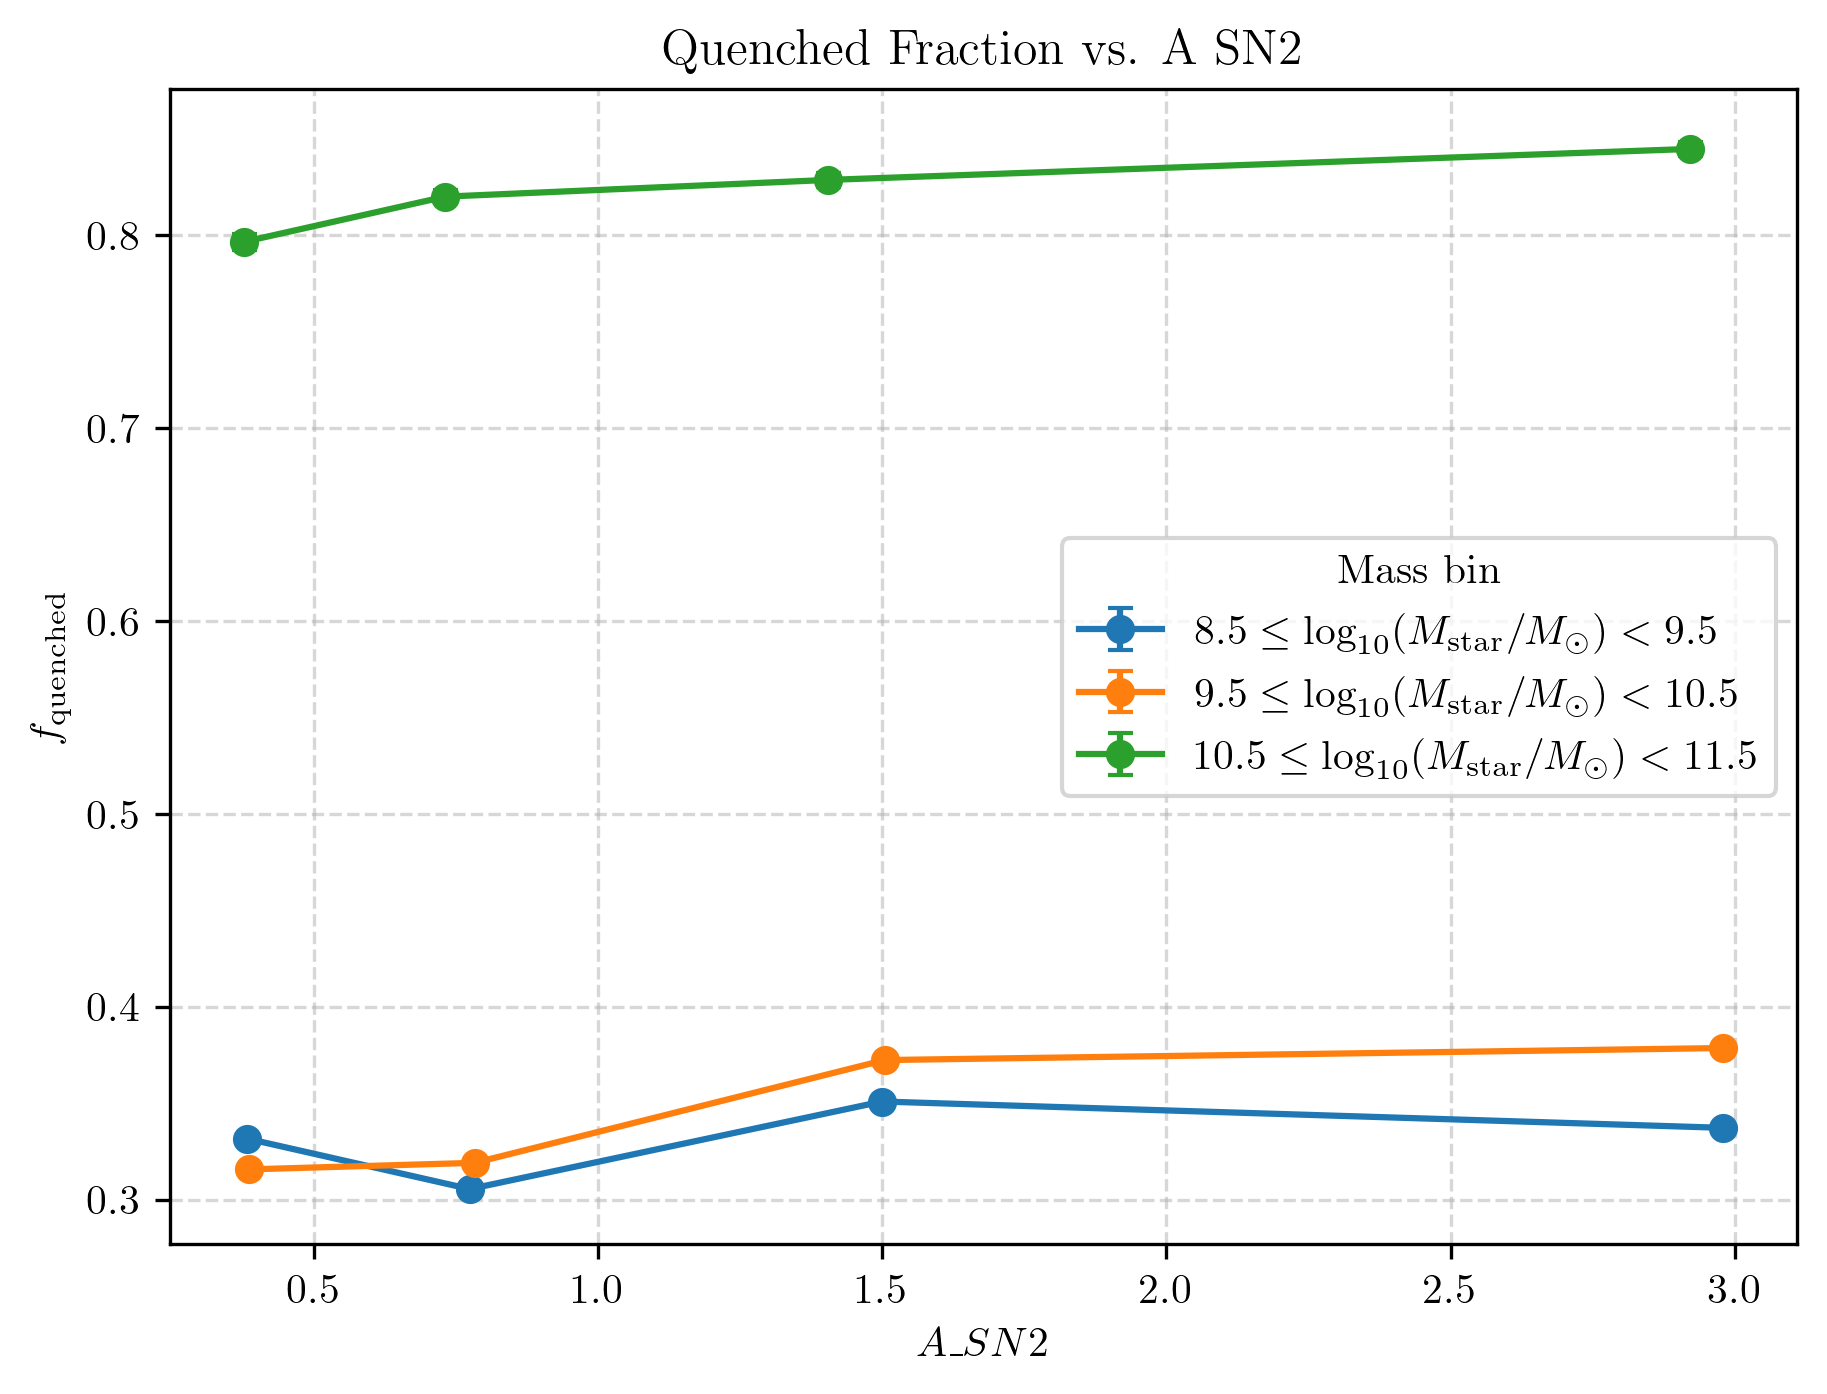
\includegraphics[width=0.5\textwidth]{../Project6/plots/fquenched_vs_A_SN2_20250424_133824.png}
    \caption{\label{fig:fquenched_ASN2} The figure displays the quenched fraction as a function of $A_{SN2}$ for three different stellar mass bins. The quenched fraction increases with stellar mass, with galaxies in the highest mass bin ($10.5 \leq \log_{10}(M_{star}/M_{\odot}) < 11.5$) showing a consistently high quenched fraction across all values of $A_{SN2}$. The quenched fraction shows a weak dependence on $A_{SN2}$ for each mass bin.
}
\end{figure}

\begin{figure}[h!]
    \centering
    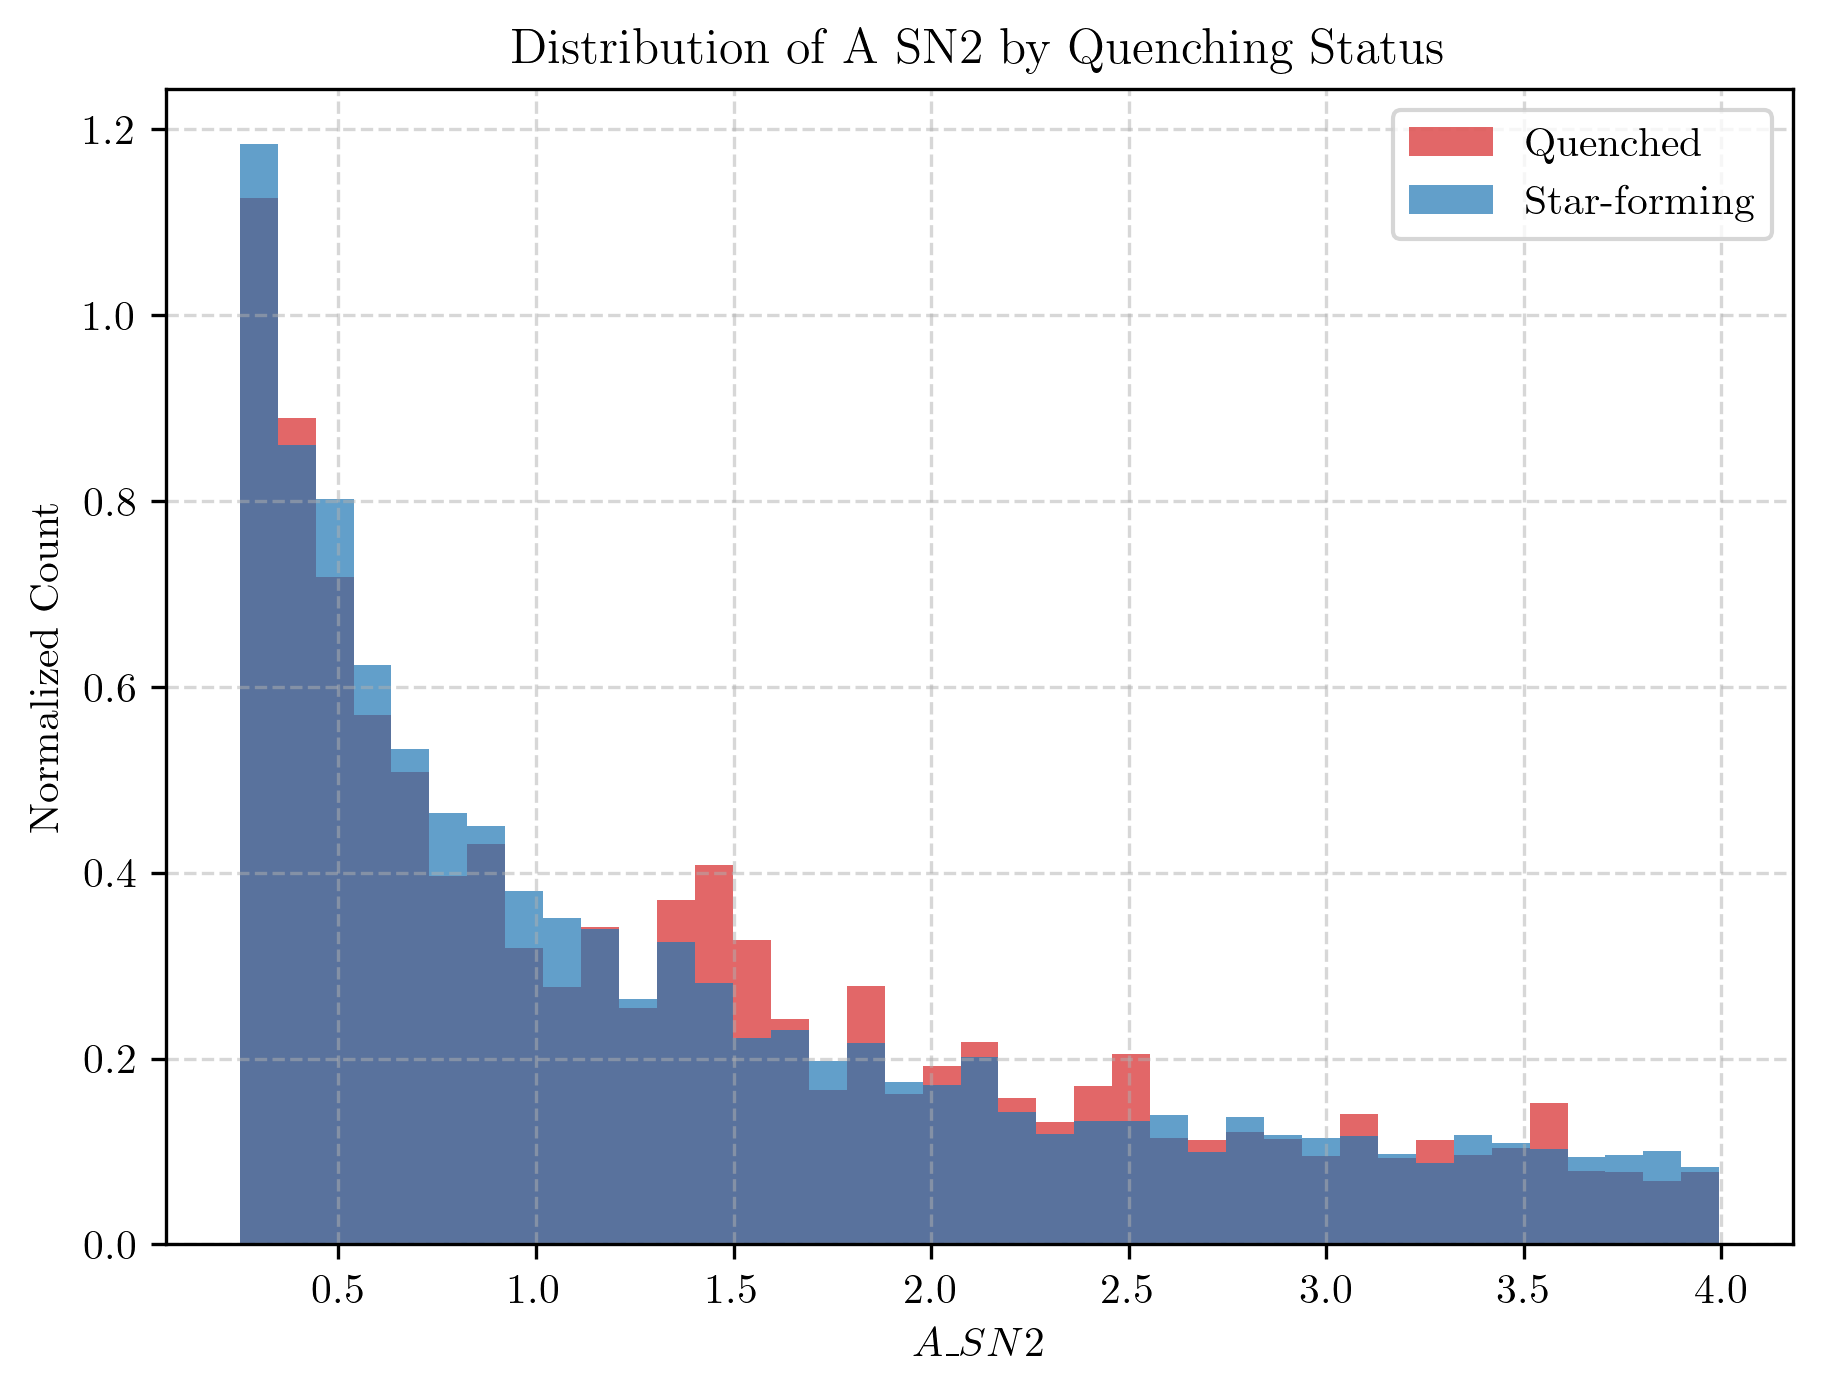
\includegraphics[width=0.5\textwidth]{../Project6/plots/A_SN2_histogram_4_20250424_133143.png}
    \caption{\label{fig:ASN2_hist} The distribution of $A_{SN2}$ is shown for both quenched and star-forming galaxies. The distributions show that star-forming galaxies have a higher density at smaller $A_{SN2}$ values than quenched galaxies.
}
\end{figure}

\begin{figure}[h!]
    \centering
    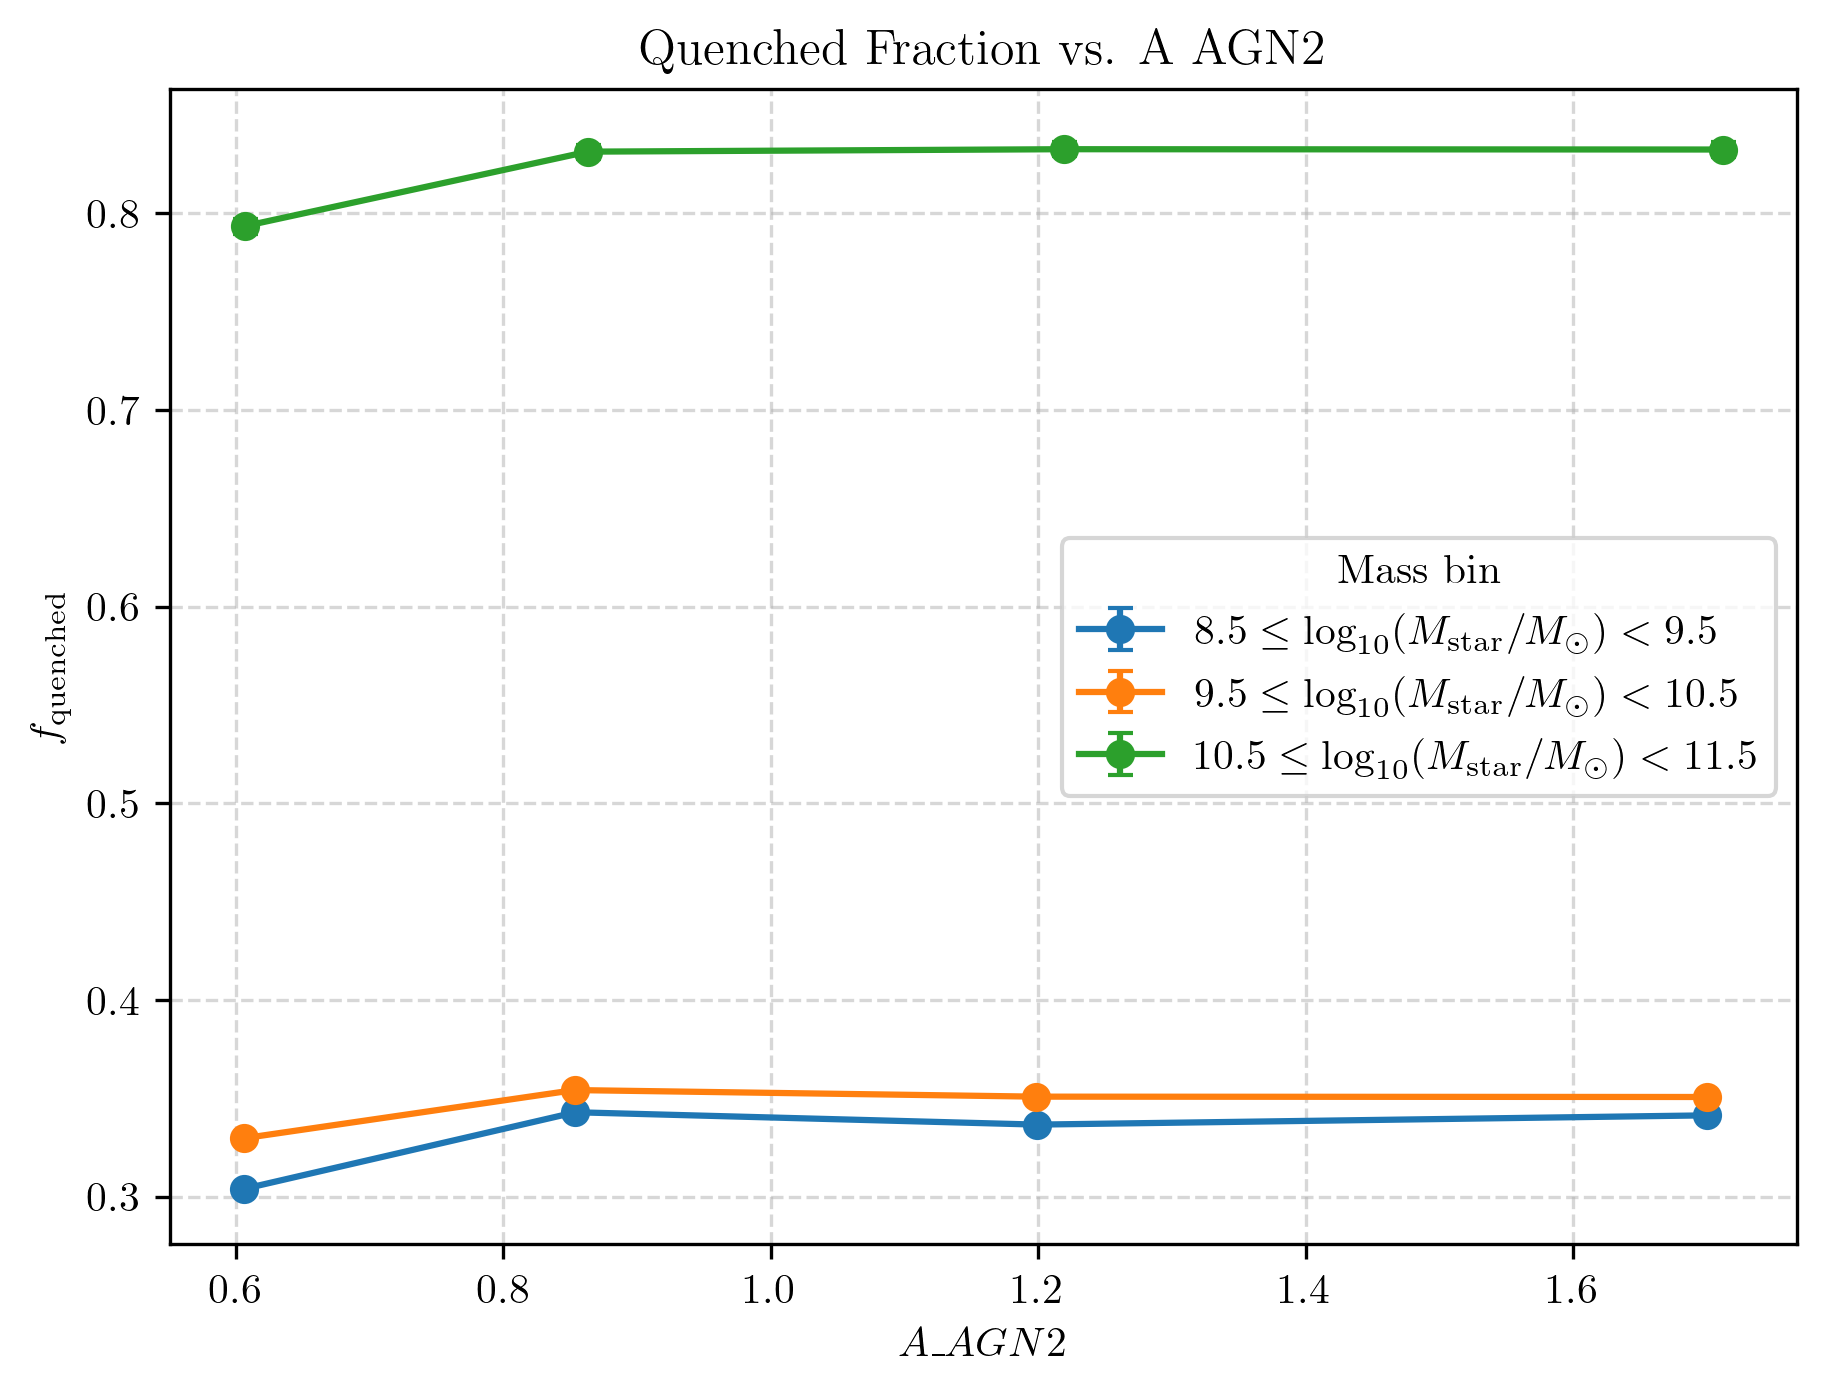
\includegraphics[width=0.5\textwidth]{../Project6/plots/fquenched_vs_A_AGN2_20250424_133935.png}
    \caption{\label{fig:fquenched_AAGN2} The quenched fraction as a function of $A_{AGN2}$ for different stellar mass bins is shown. The quenched fraction is significantly higher for galaxies in the highest mass bin ($10.5 \leq \log_{10}(M_{star}/M_{\odot}) < 11.5$) compared to the lower mass bins. The quenched fraction appears to be relatively constant as a function of $A_{AGN2}$ for each mass bin.
}
\end{figure}

\begin{figure}[h!]
    \centering
    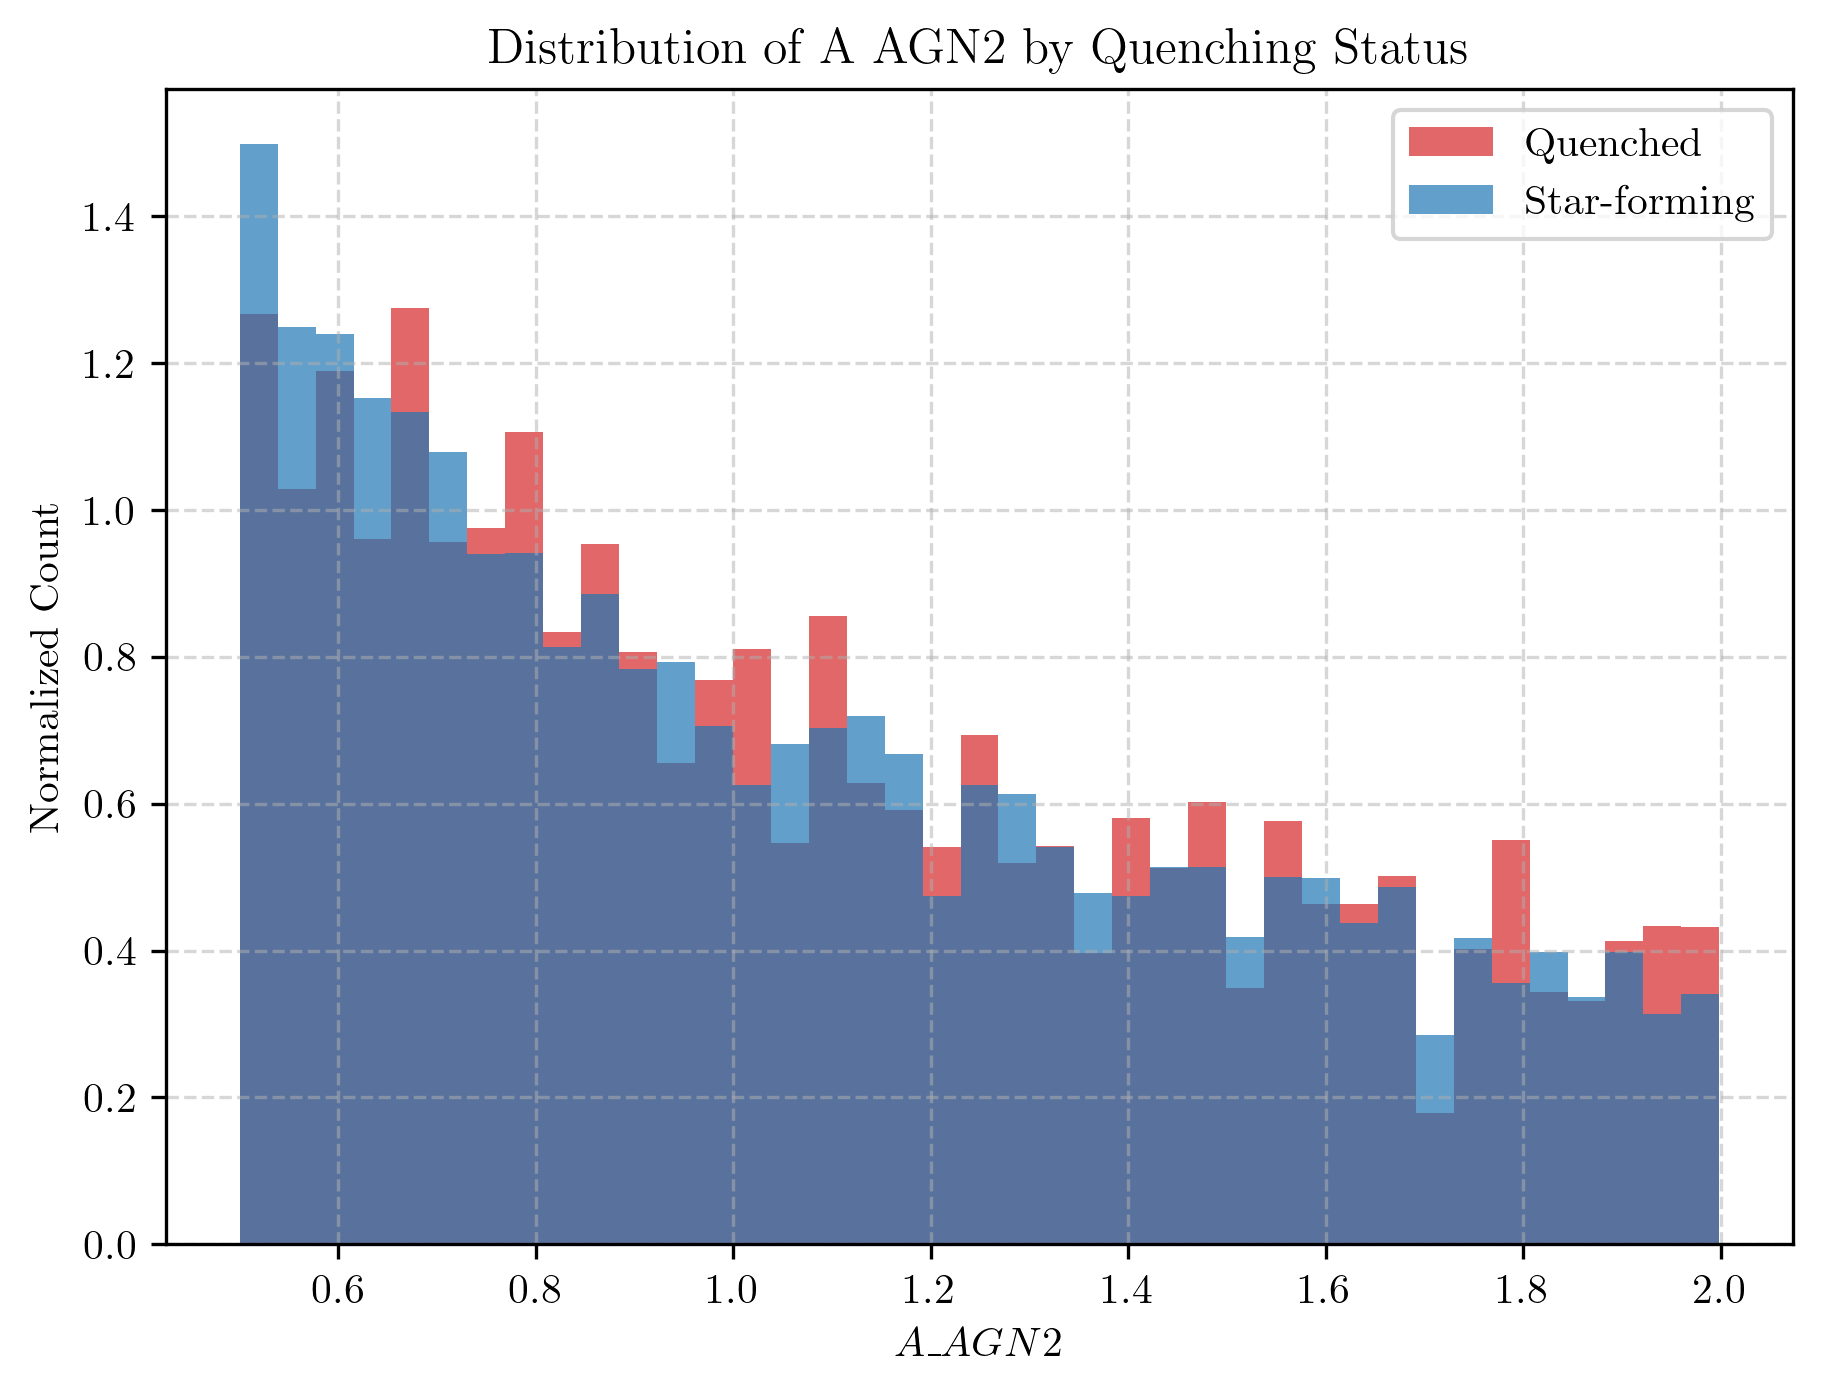
\includegraphics[width=0.5\textwidth]{../Project6/plots/A_AGN2_histogram_6_20250424_133143.png}
    \caption{\label{fig:AAGN2_hist} Distribution of $A\_AGN2$ for quenched and star-forming galaxies. The normalized count is plotted against $A\_AGN2$. Overall, the star-forming galaxies tend to have slightly smaller $A\_AGN2$ values compared to quenched galaxies, but the differences are relatively small with significant overlap in the distributions.
}
\end{figure}

\subsubsection{Cosmological Parameters}

The cosmological parameters \(\Omega_m\) (matter density parameter) and \(\sigma_8\) (power spectrum normalization) also influence the quenched fraction. Higher values of both parameters are associated with an increased \(f_{quenched}\). This is consistent with the idea that denser cosmic environments and enhanced clustering, leading to earlier structure formation, favor quenching processes such as accelerated black hole growth and the formation of more massive halos, which more efficiently host quenching mechanisms.

\subsection{Statistical Modeling and Feature Importance}

To quantify the relative importance of each parameter in predicting galaxy quenching, we employ a logistic regression model. The target variable is a binary flag indicating whether a galaxy is quenched (sSFR \(< 10^{-11} \text{ yr}^{-1}\)). We use permutation feature importance to assess the contribution of each parameter to the model's performance.

\subsubsection{Permutation Feature Importance}

The permutation feature importance analysis reveals that \(\sigma_8\) is the most important parameter (importance mean \(\sim\)0.155), followed by \(A_{AGN1}\) (\(\sim\)0.148), \(\Omega_m\) (\(\sim\)0.128), and the logarithm of stellar mass (\(\log M_{star}\), \(\sim\)0.104). The supernova feedback parameter \(A_{SN1}\) also exhibits significant importance (\(\sim\)0.094). These results are summarized in Figure \ref{fig:permutation_importance}, which shows the permutation feature importances for all parameters. These results underscore the combined influence of cosmological environment, AGN feedback, and stellar mass on galaxy quenching.

\begin{figure}[h!]
    \centering
    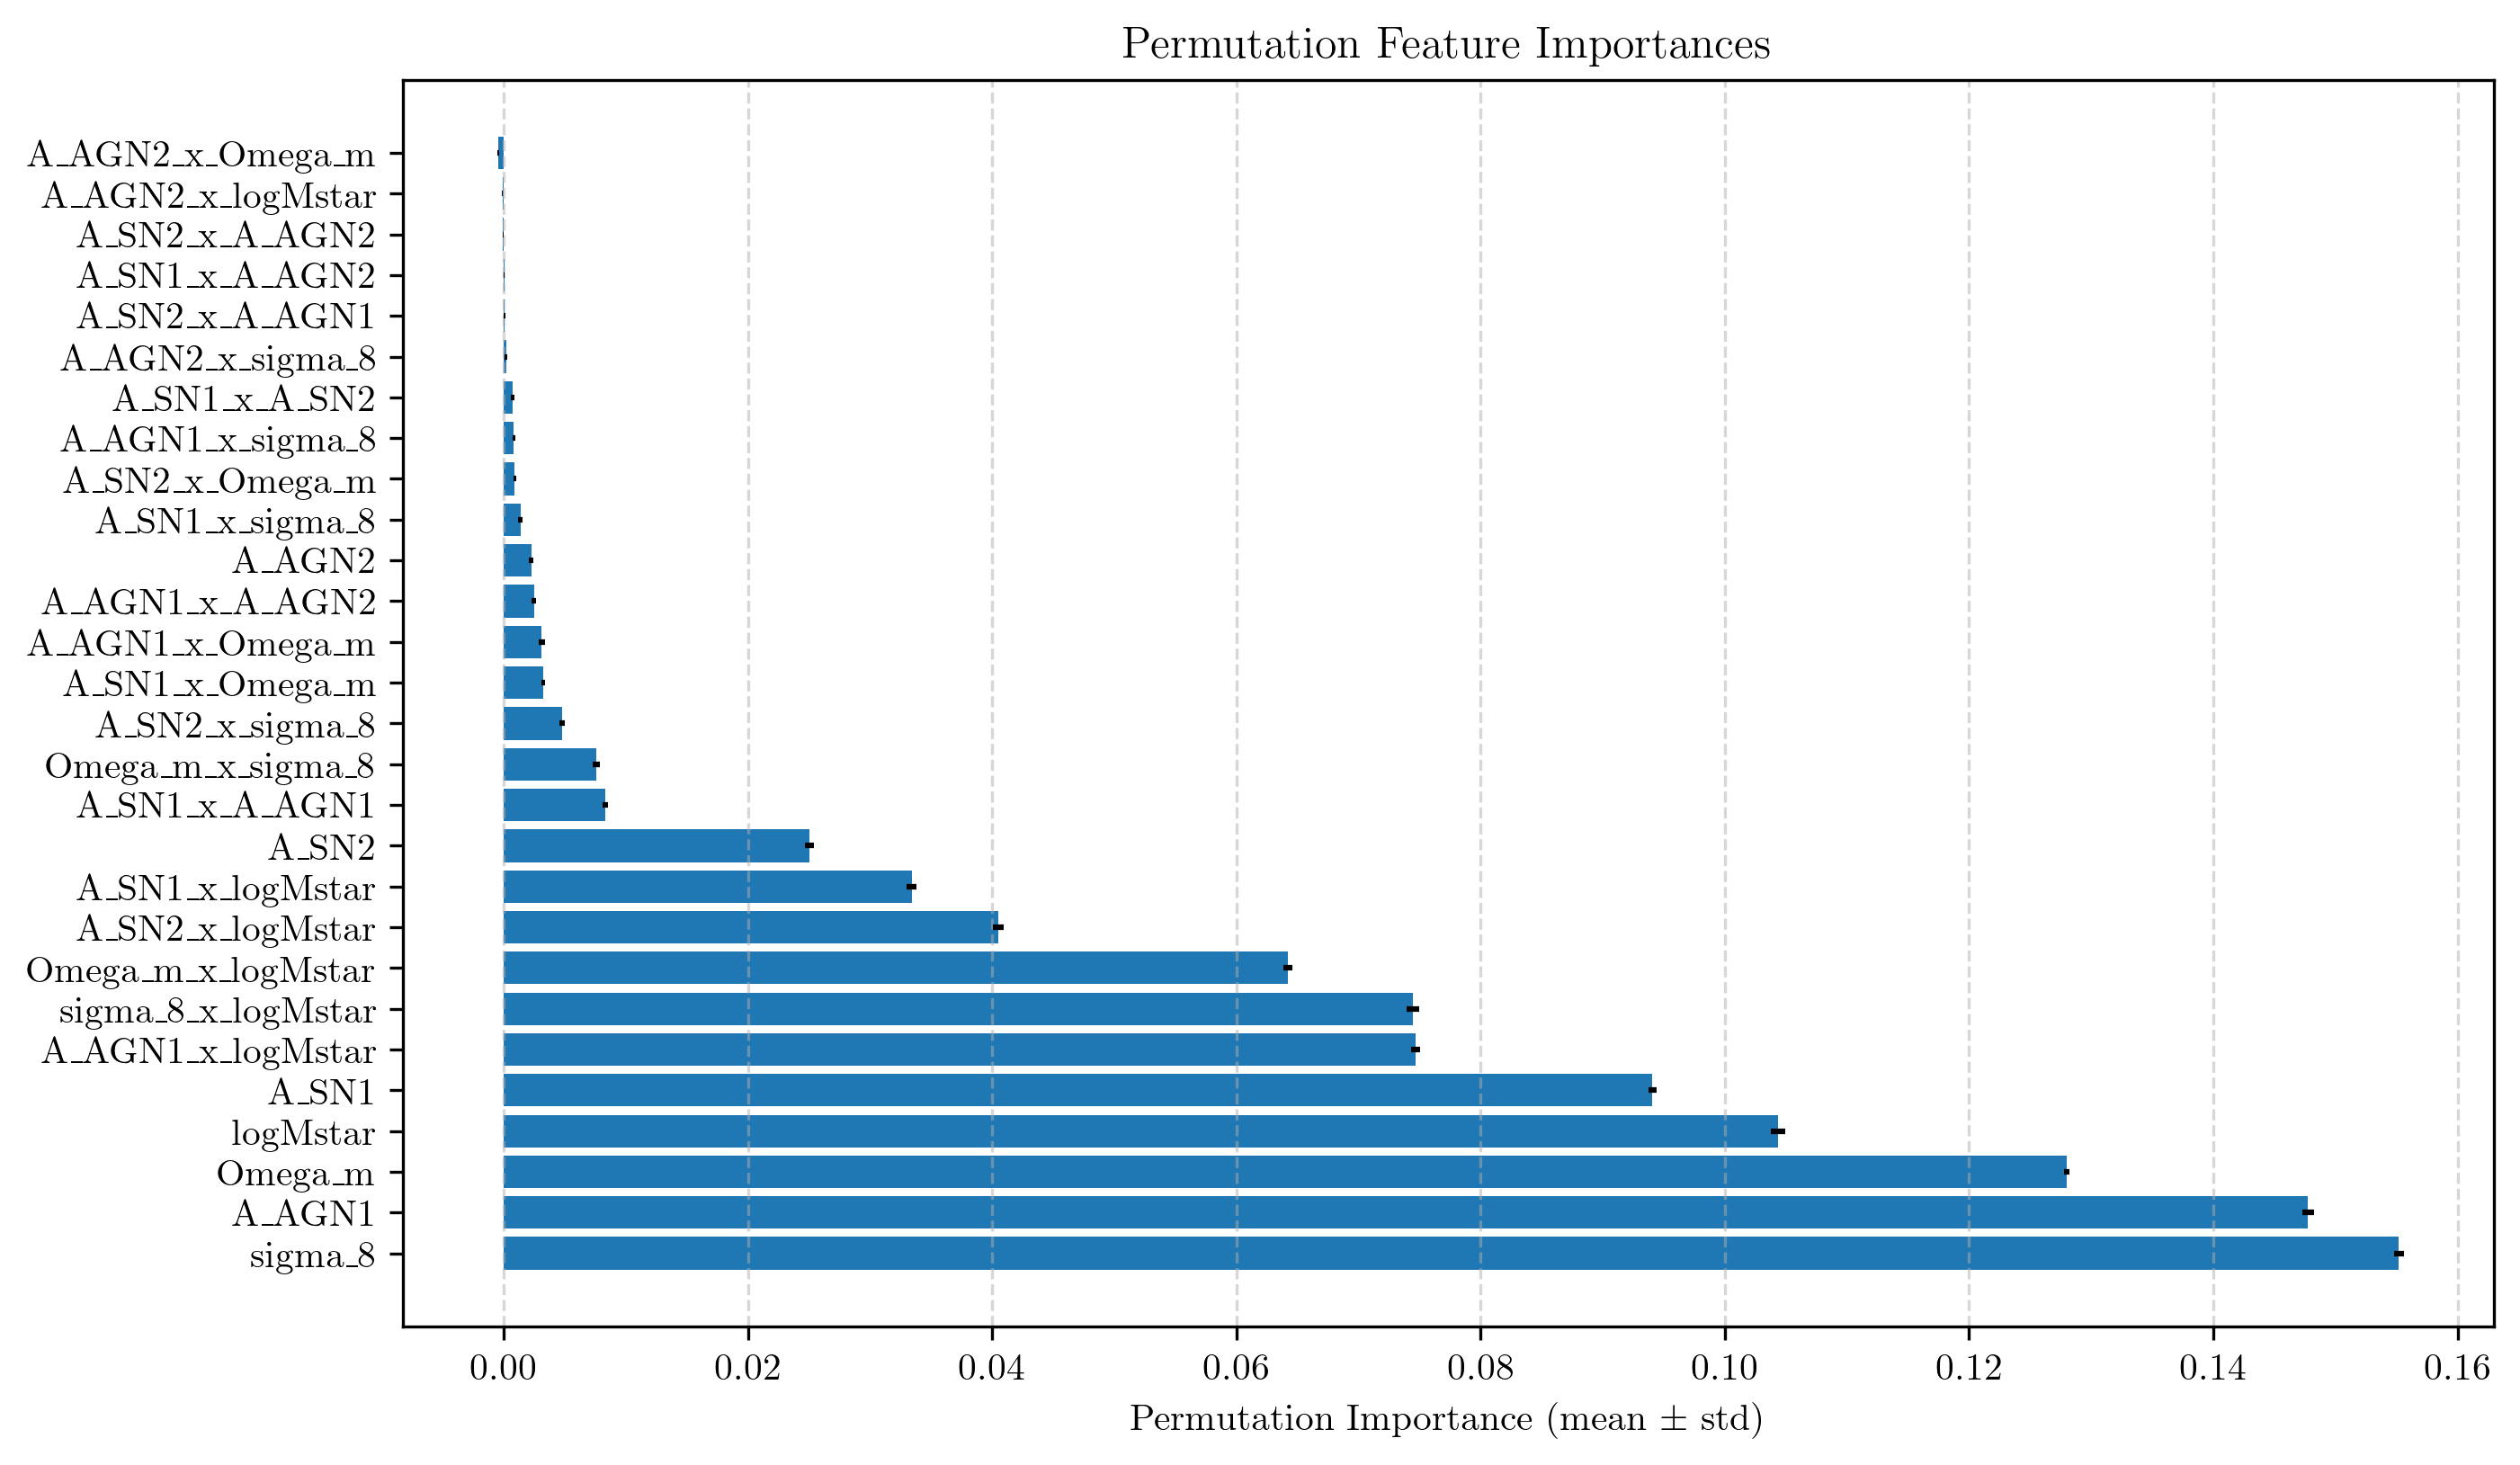
\includegraphics[width=0.5\textwidth]{../Project6/plots/permutation_importance_20250424_133935.png}
    \caption{\label{fig:permutation_importance} The figure displays the permutation feature importances, quantifying the contribution of different features and their combinations to the model's performance. The x-axis represents the permutation importance (mean $\pm$ std), while the y-axis lists the features. The features "sigma\_8", "A\ensuremath{\_}AGN1", "Omega\_m", "logMstar", and "A\ensuremath{\_}SN1" show the largest permutation importance.
}
\end{figure}

\subsubsection{Logistic Regression Coefficients}

The coefficients of the logistic regression model further highlight the key drivers of quenching. The coefficients are shown in Figure \ref{fig:logreg_coefficients}. \(A_{AGN1}\) has a strong positive coefficient (+1.87), indicating a strong positive association with quenching. Similarly, \(\sigma_8\) (+1.66), \(\log M_{star}\) (+1.41), and \(\Omega_m\) (+1.13) also have positive coefficients. In contrast, \(A_{SN1}\) has a negative coefficient (–0.97), reflecting its role in suppressing quenching. The magnitudes of these coefficients emphasize the substantial impact of AGN feedback and cosmological parameters on driving galaxy quenching.

\begin{figure}[h!]
    \centering
    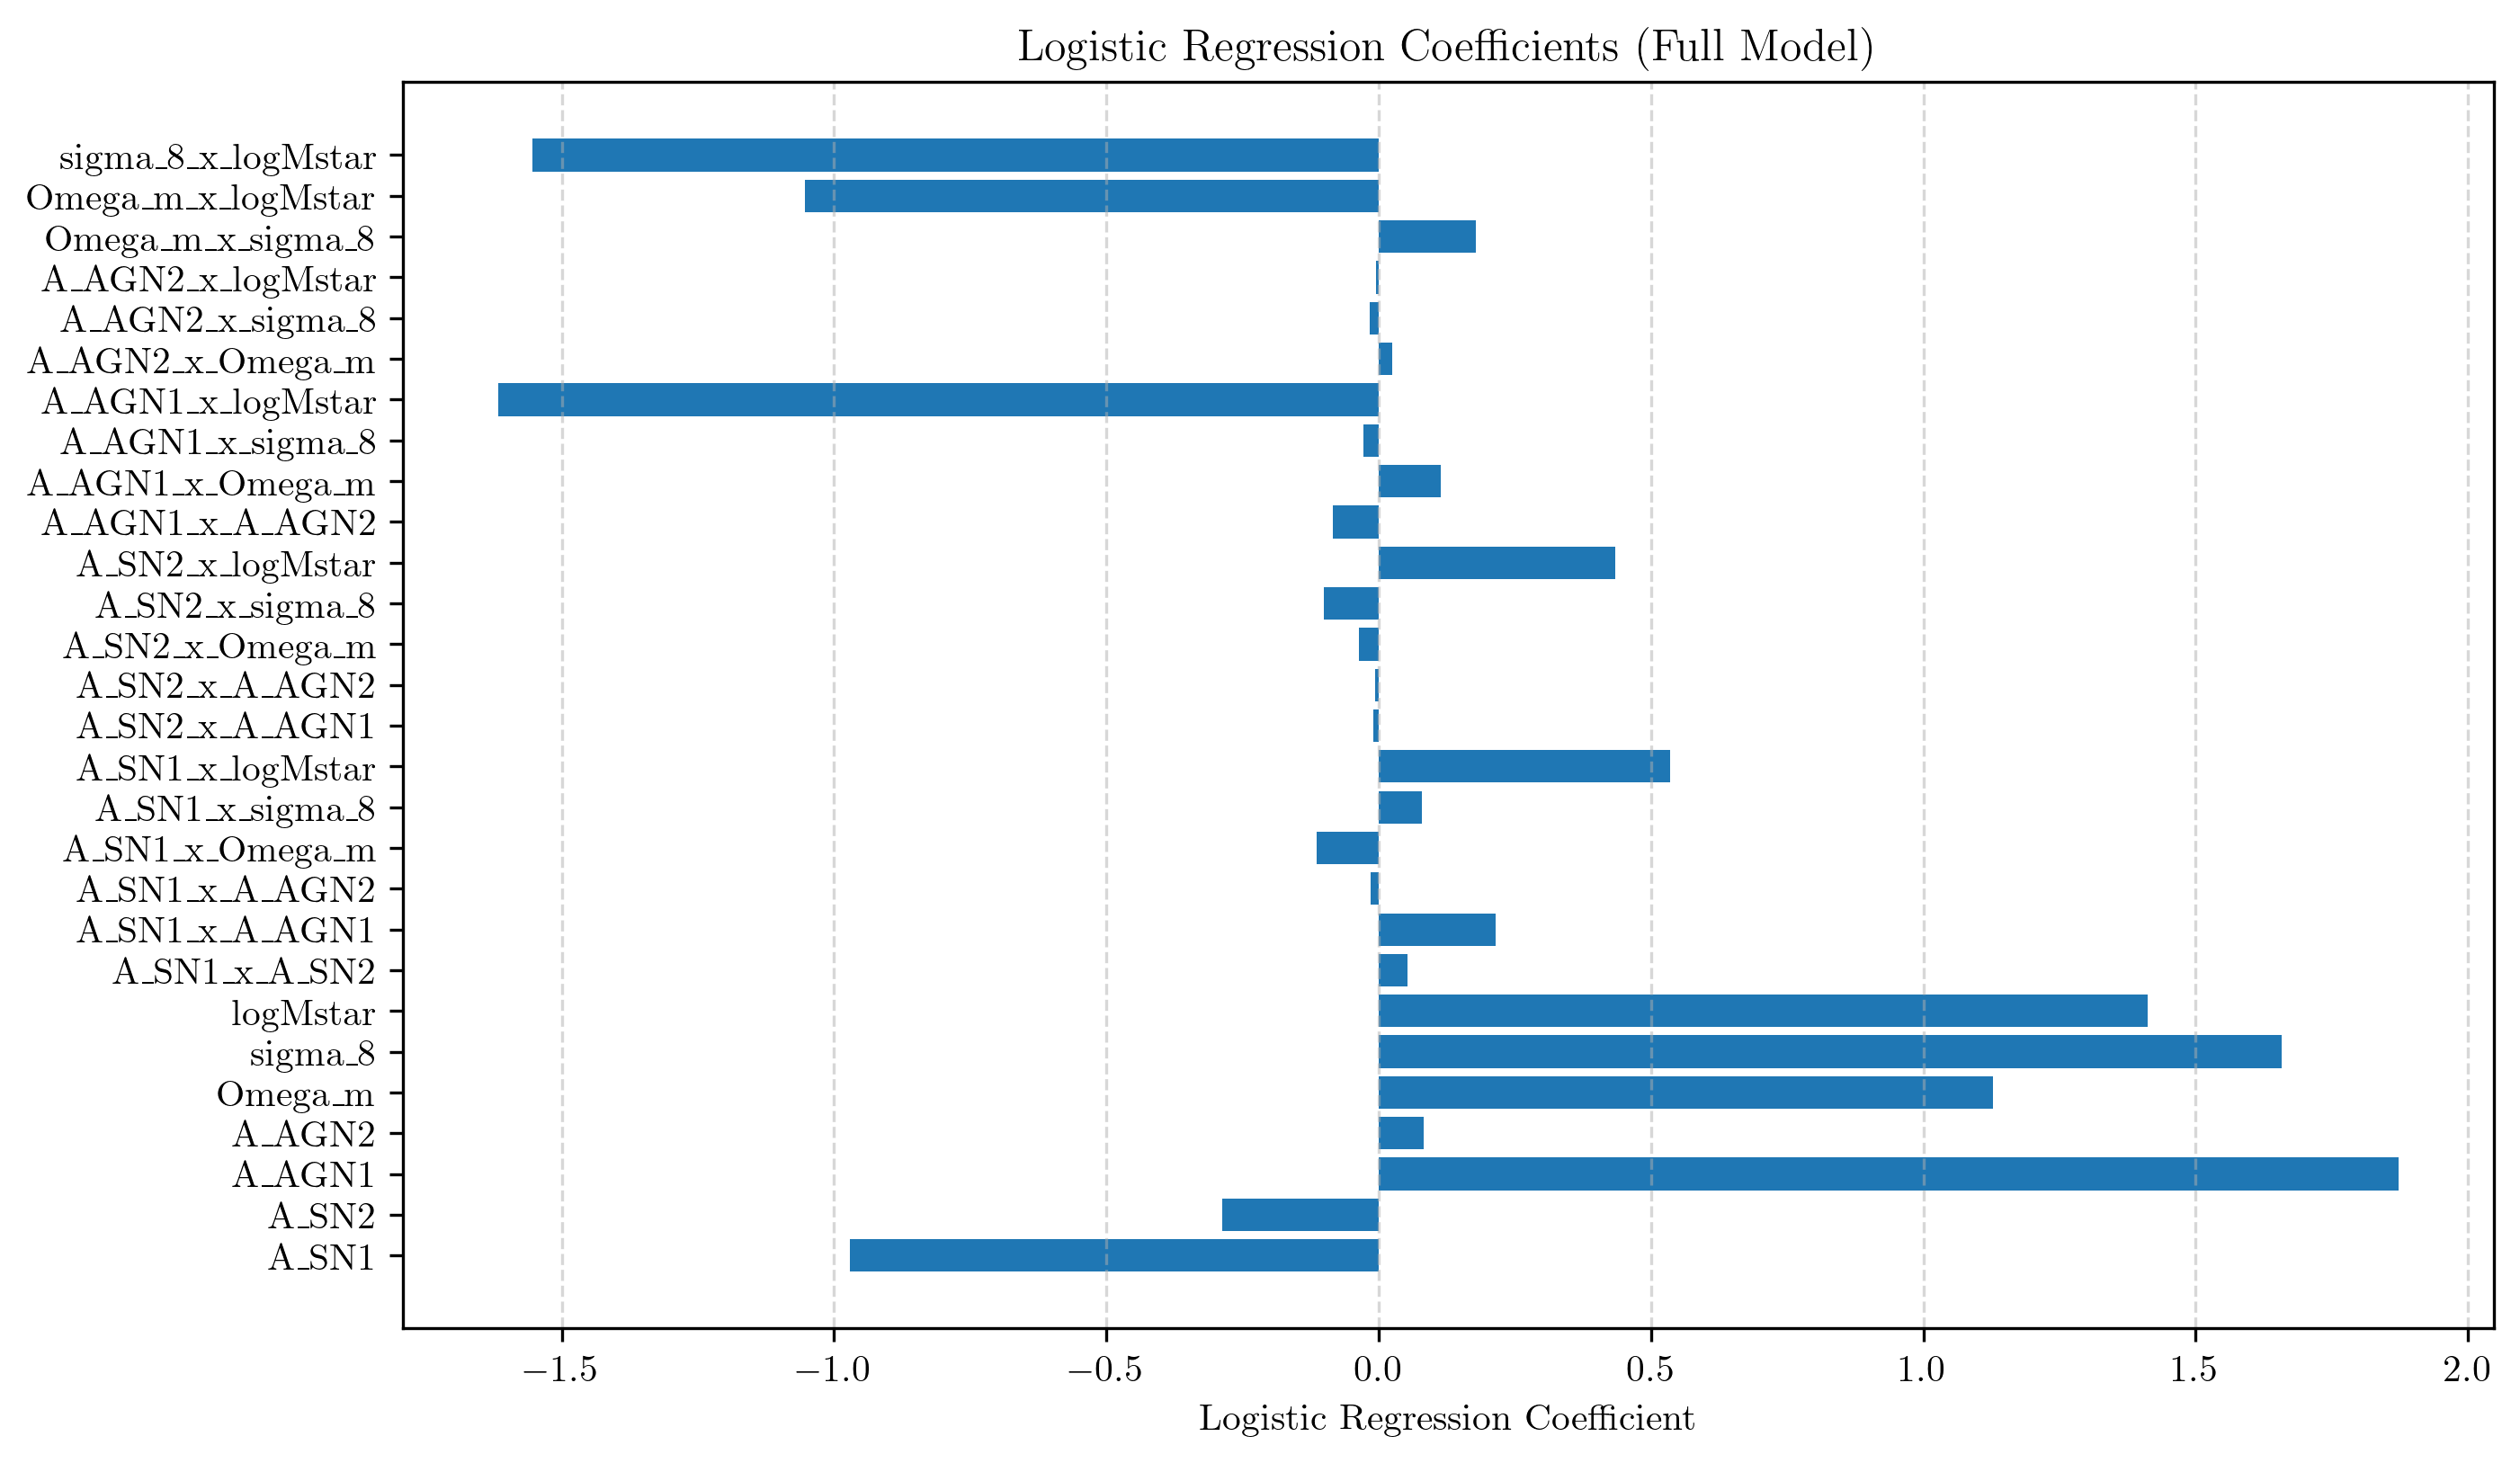
\includegraphics[width=0.5\textwidth]{../Project6/plots/logreg_coefficients_20250424_133935.png}
    \caption{\label{fig:logreg_coefficients} The figure shows the Logistic Regression Coefficients for the full model. Large differences are seen in the magnitude and sign of the coefficients, indicating varying degrees of influence from different combinations of cosmological parameters (e.g., $\sigma_8$, $\Omega_m$, $logMstar$) and survey parameters (A\ensuremath{\_}SN1, A\ensuremath{\_}SN2, A\ensuremath{\_}AGN1, A\ensuremath{\_}AGN2) on the logistic regression model.
}
\end{figure}

\subsubsection{Partial Correlations}

Partial correlation analysis, which measures the correlation between two variables while controlling for the effects of other variables, confirms the results obtained from the regression analysis. \(A_{AGN1}\), \(\sigma_8\), and \(\Omega_m\) exhibit positive partial correlations with quenching (with values around +0.15, +0.16, and +0.14, respectively), while \(A_{SN1}\) shows a negative partial correlation (–0.11).

\subsubsection{Model Performance}

The full logistic regression model, including all parameters and their interactions, achieves a mean accuracy of approximately 66.5\% and an area under the receiver operating characteristic curve (AUC) of approximately 0.685. A simplified model using only the top three most important features (\(\sigma_8\), \(A_{AGN1}\), and \(\Omega_m\)) yields slightly lower performance (accuracy \(\sim\)64.5\% and AUC \(\sim\)0.645). This suggests that the majority of the predictive power is concentrated in a few key parameters, though the inclusion of other parameters does provide some additional predictive power.

\subsection{Mass Dependence and Parameter Interplay}

The analysis reveals that the dominant quenching mechanisms differ across stellar mass ranges. AGN feedback appears to be the primary driver of quenching in high-mass galaxies, while SN feedback plays a more regulatory role in low to intermediate mass systems.

To further explore the interplay between parameters, we generate two-dimensional heatmaps showing the quenched fraction as a function of pairs of parameters. Figure \ref{fig:heatmap_fquenched} shows the heatmap of the quenched fraction as a function of $A_{AGN1}$ and $A_{SN1}$ for galaxies with stellar masses in the range $8.5 \leq \log_{10}(M_{\rm star}/M_{\odot}) < 9.5$. Figure \ref{fig:heatmap_fquenched_2} and Figure \ref{fig:heatmap_fquenched_3} show the same heatmap for galaxies with stellar masses in the range $9.5 \leq \log_{10}(M_{\star}/M_{\odot}) < 10.5$ and $10.5 \leq \log_{10}(M_{\star}/M_{\odot}) < 11.5$, respectively. These visualizations indicate that the highest quenched fractions occur in regions where \(A_{AGN1}\) is high and \(A_{SN1}\) is low. This suggests a synergistic effect, where quenching is most efficient when AGN feedback is strong and SN feedback is weak. This also suggests that the quenching is not simply a linear combination of the effects of the parameters, but that there are non-linear interactions between them.

\begin{figure}[h!]
    \centering
    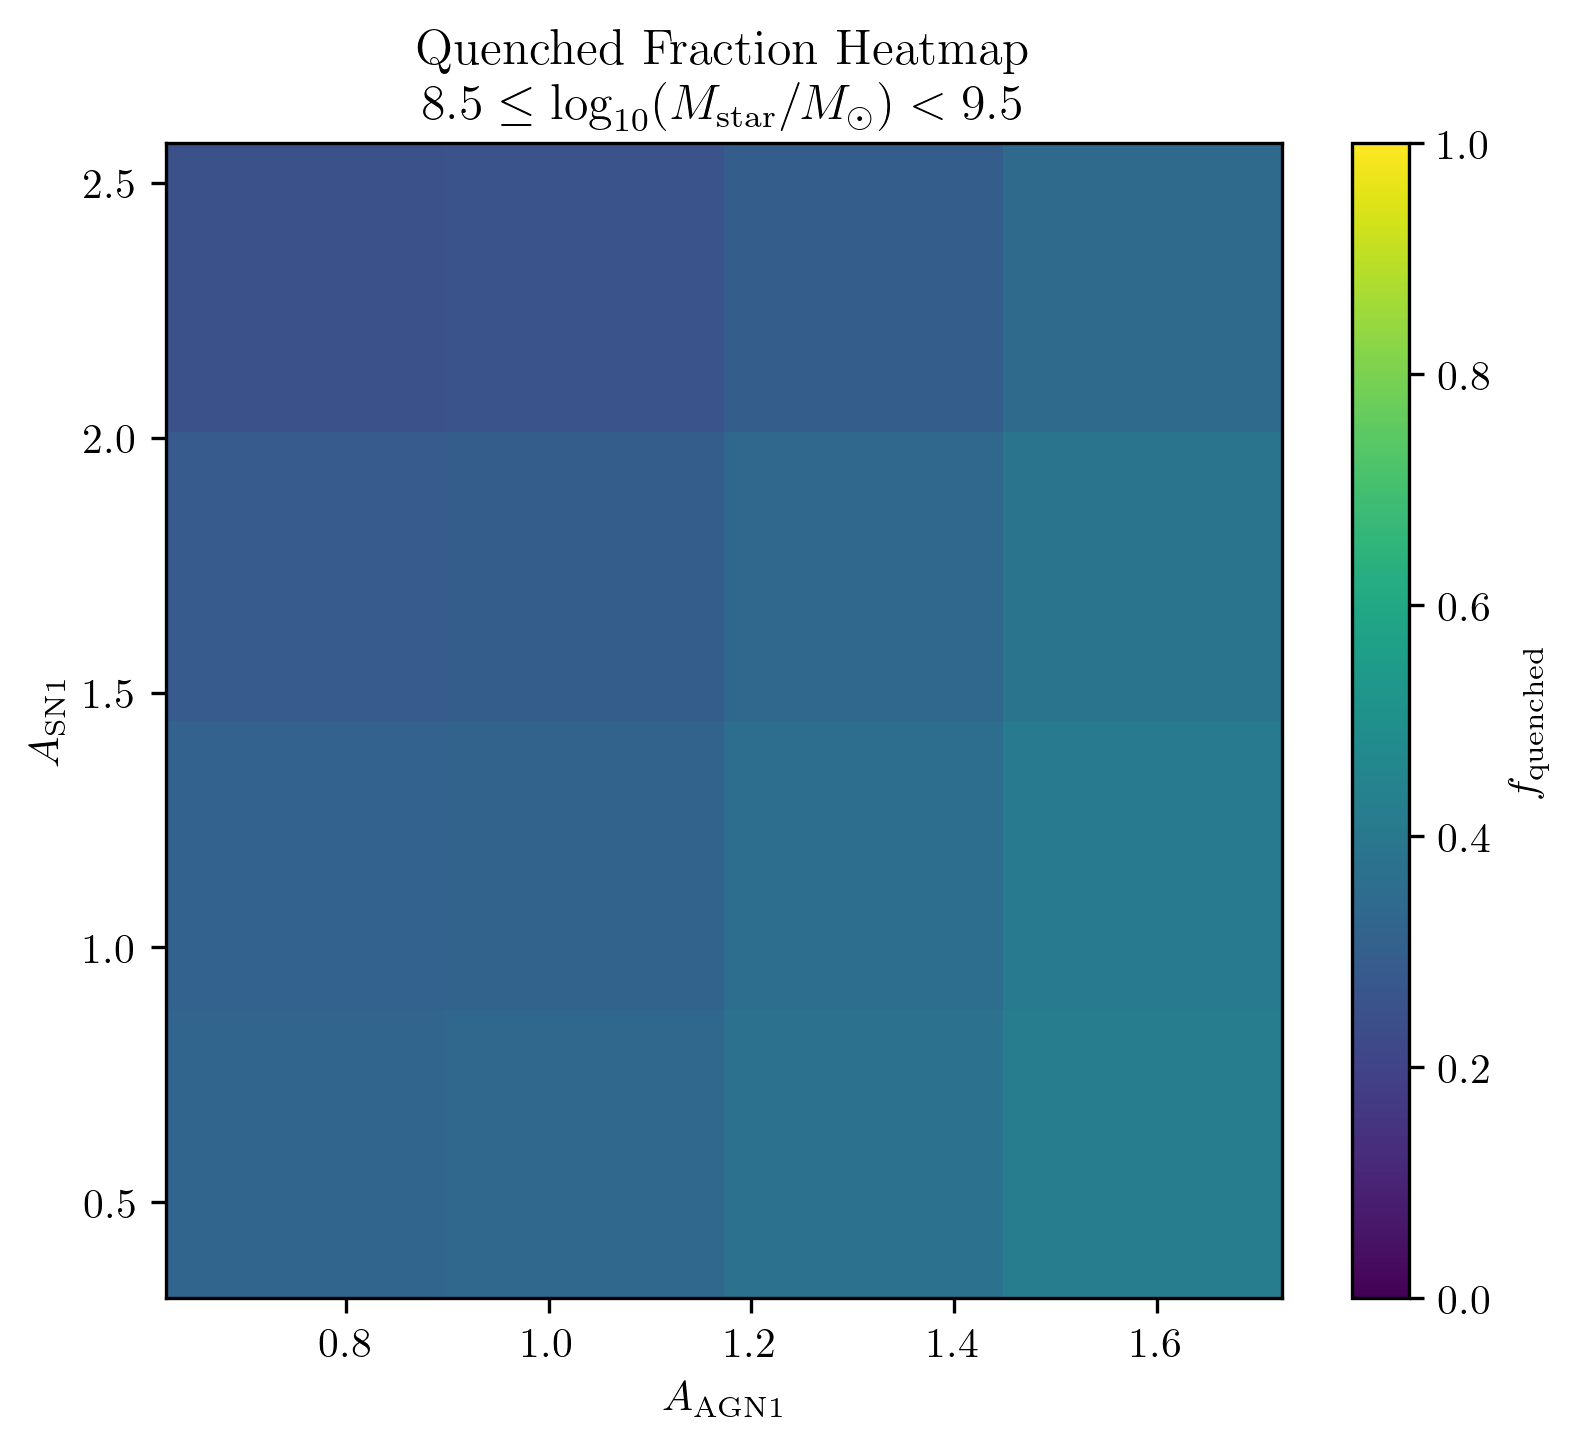
\includegraphics[width=0.5\textwidth]{../Project6/plots/fquenched_heatmap_SN1_AGN1_8_5_10_M_star_M_9_5_20250424_133935.png}
    \caption{\label{fig:heatmap_fquenched} Heatmap of the quenched fraction ($f_{\rm quenched}$) as a function of $A_{\rm AGN1}$ and $A_{\rm SN1}$ for galaxies with stellar masses in the range $8.5 \leq \log_{10}(M_{\rm star}/M_{\odot}) < 9.5$. The quenched fraction increases with increasing $A_{\rm AGN1}$ and *decreasing* $A_{\rm SN1}$, with a more pronounced increase along the $A_{\rm AGN1}$ axis.
}
\end{figure}

\begin{figure}[h!]
    \centering
    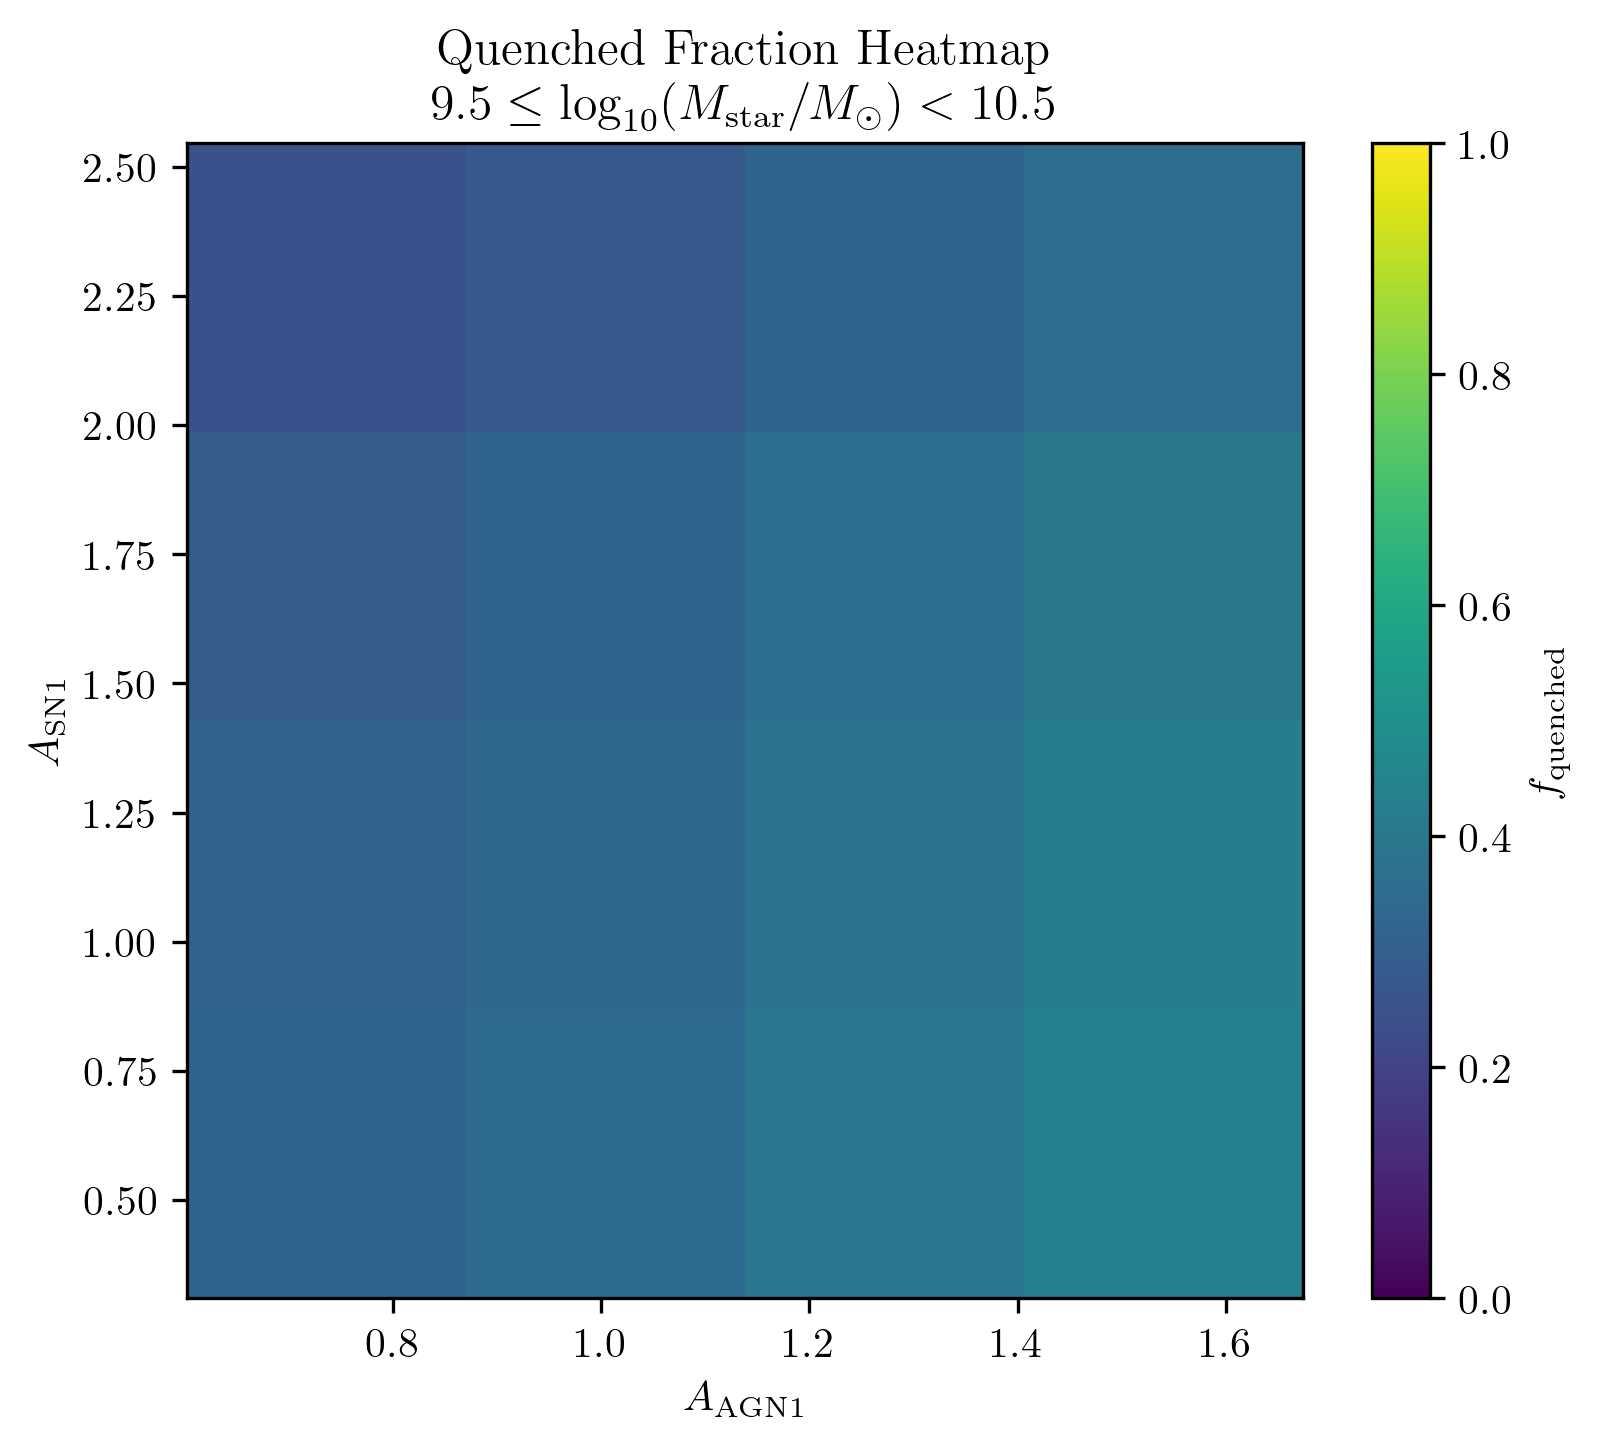
\includegraphics[width=0.5\textwidth]{../Project6/plots/fquenched_heatmap_SN1_AGN1_9_5_10_M_star_M_10_5_20250424_133935.png}
    \caption{\label{fig:heatmap_fquenched_2} Quenched fraction heatmap for galaxies with stellar masses in the range $9.5 \leq \log_{10}(M_{\star}/M_{\odot}) < 10.5$. The x-axis represents $A_{AGN1}$ and the y-axis represents $A_{SN1}$. The colorbar indicates the quenched fraction, $f_{\mathrm{quenched}}$. The quenched fraction increases as you move towards larger values of $A_{AGN1}$.
}
\end{figure}

\begin{figure}[h!]
    \centering
    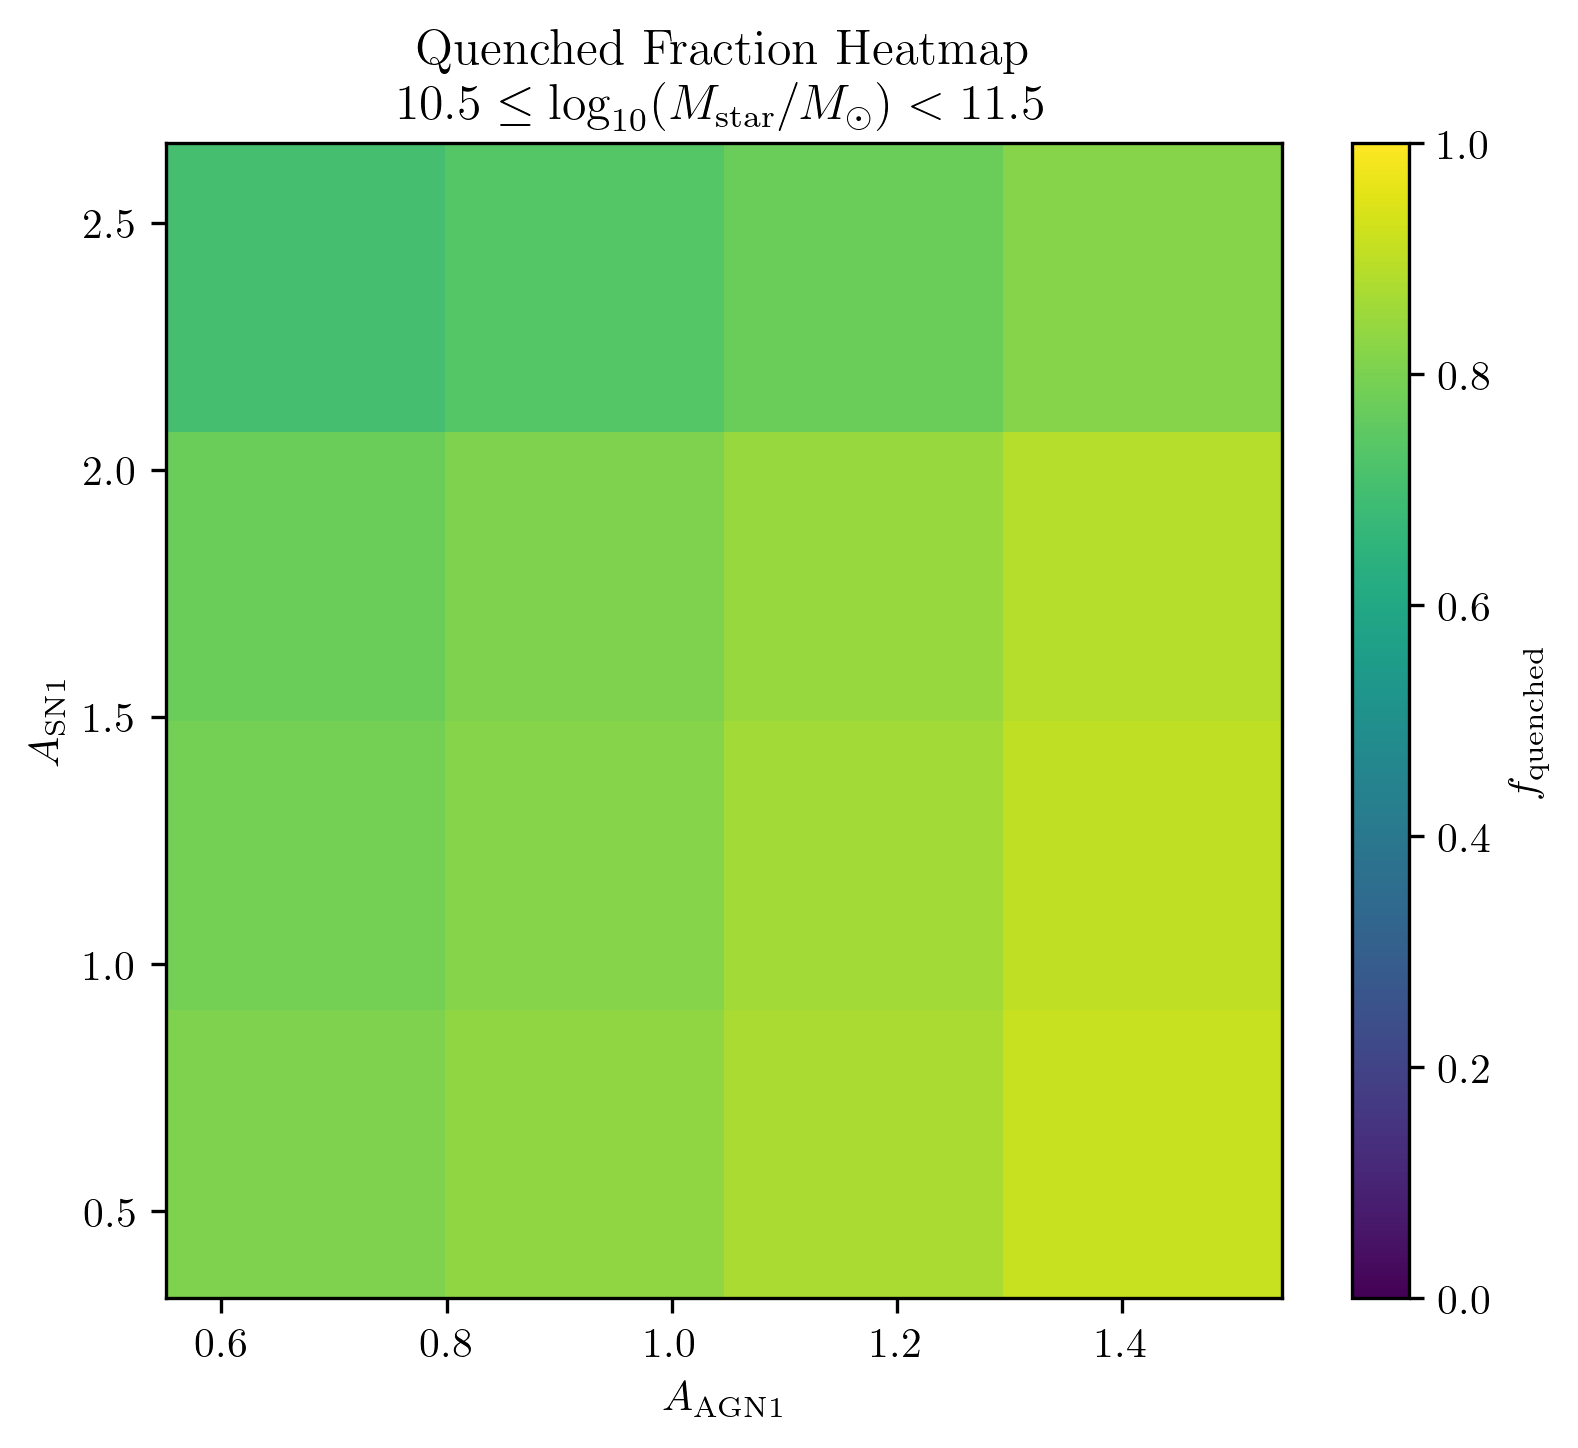
\includegraphics[width=0.5\textwidth]{../Project6/plots/fquenched_heatmap_SN1_AGN1_10_5_10_M_star_M_11_5_20250424_133935.png}
    \caption{\label{fig:heatmap_fquenched_3} Quenched fraction of galaxies with stellar mass $10.5 \leq \log_{10}(M_{\star}/M_{\odot}) < 11.5$ as a function of $A_{\rm AGN1}$ and $A_{\rm SN1}$. The quenched fraction increases with increasing $A_{\rm AGN1}$.
}
\end{figure}

\section{Conclusions}
\label{sec:conclusions}


In this study, we have systematically investigated the efficiency of star formation quenching across a wide range of feedback and cosmological parameters using the CAMELS simulations. Our primary goal was to disentangle the complex interplay between supernova (SN) feedback, active galactic nucleus (AGN) feedback, and cosmological parameters in driving the cessation of star formation in galaxies at $z=0$. By leveraging the extensive parameter space coverage of the CAMELS simulations, we aimed to provide quantitative insights into the physical drivers of quenching and offer predictive guidance for galaxy evolution models and future observational surveys.

We utilized galaxy-level data from the IllustrisTNG and SIMBA simulation suites within CAMELS, focusing on key parameters such as SN feedback efficiency (\(A_{SN1}\), \(A_{SN2}\)), AGN feedback efficiency (\(A_{AGN1}\), \(A_{AGN2}\)), matter density parameter (\(\Omega_m\)), and the amplitude of the matter power spectrum (\(\sigma_8\)). We calculated the quenched fraction (\(f_{quenched}\)) for galaxies in different stellar mass bins and explored the dependence of \(f_{quenched}\) on the aforementioned parameters. Statistical techniques, including permutation feature importance, logistic regression, and partial correlation analysis, were employed to quantify the relative importance of each parameter and to uncover potential interactions.

Our results reveal a nuanced picture of galaxy quenching. We found that AGN feedback, particularly the AGN feedback energy per accretion (\(A_{AGN1}\)), is the dominant quenching mechanism in massive galaxies, while SN feedback exhibits a more regulatory effect in lower-mass systems. Specifically, an increase in \(A_{AGN1}\) correlates with a higher quenched fraction, especially in galaxies with \(\log_{10}(M_{star}/M_\odot) \geq 10.5\). Conversely, higher SN wind energy (\(A_{SN1}\)) tends to *decrease* the quenched fraction in low to intermediate mass galaxies. Furthermore, we observed that cosmological parameters (\(\Omega_m\) and \(\sigma_8\)) positively influence quenching efficiency, suggesting that denser cosmic environments and enhanced clustering promote quenching.

From this study, we have learned that the efficiency of star formation quenching is not solely determined by internal feedback processes but is also significantly influenced by the broader cosmological context. The interplay between AGN feedback, SN feedback, and cosmological parameters is complex and nonlinear, with stellar mass acting as a crucial modulator. Our findings underscore the importance of accurately representing AGN feedback in galaxy evolution models, particularly for massive galaxies, and of considering the environmental context when studying quenching. The results also suggest that future models should adopt a joint, nonlinear approach to capture the synergistic effects that operate across different mass regimes.

In conclusion, our analysis of the CAMELS simulations provides a comprehensive map of star formation quenching efficiency across feedback and cosmological parameter space. We have demonstrated that AGN feedback, SN feedback, and cosmological parameters all play significant, interconnected roles in driving the cessation of star formation in galaxies. These findings offer valuable insights for refining galaxy evolution models and interpreting observational data from future surveys.
\

\bibliography{bibliography}{}
\bibliographystyle{aasjournal}

\end{document}
